%% =====================================================================================
%%  INTEGRATED MANUSCRIPT -- target: Artificial Intelligence in Medicine (Elsevier, hybrid;
%%  subscription route, no APC). On Overleaf: \documentclass[preprint,12pt]{elsarticle} and
%%  move the author block into \author/\affiliation; body unchanged. Word budget ~9,500 incl.
%%  captions (AIIM has no hard page limit; this is ~15 pp. in this layout, ~28 pp. preprint).
%%  Tables/figures are generated by code (results/real/*, scripts/*). Red = to be confirmed by
%%  the authors (Part I full-text verification, registration IDs, funding).
%% =====================================================================================
\documentclass[11pt,a4paper]{article}
\usepackage[T1]{fontenc}\usepackage[utf8]{inputenc}\usepackage{lmodern}\usepackage{microtype}
\usepackage[margin=2.3cm]{geometry}\usepackage{booktabs}\usepackage{graphicx}\usepackage{longtable}
\usepackage{amsmath}\usepackage{tabularx}\usepackage{array}\usepackage{ragged2e}\usepackage{xcolor}
\usepackage{adjustbox}\usepackage{tikz}\usetikzlibrary{arrows.meta,positioning,calc}
\usepackage[hidelinks]{hyperref}\usepackage{lineno}\usepackage{enumitem}
\definecolor{accent}{HTML}{8C2F1E}
\graphicspath{{../empirical/figures/}{figures/}}
\makeatletter\def\input@path{{../empirical/}{./}}\makeatother
\newcolumntype{L}{>{\RaggedRight\arraybackslash}X}
\setlength{\parskip}{0.35em}\setlength{\parindent}{0pt}
\title{\large Machine Learning for Mental Disorder Detection from Actigraphy:\\
Published Claims versus Subject-wise, Cross-cohort and Calibrated Evaluation}
\author{Aminat Abiola Ajibola$^{1,*}$ \and Roger Nick Anaedevha$^{2}$}
\date{\footnotesize $^{1}$College of Computer Science and Engineering, University of Hafr Al-Batin, Eastern Province, Kingdom of Saudi Arabia \\
$^{2}$Institute of Cyber Intelligence Systems, National Research Nuclear University MEPhI, Moscow, Russian Federation \\[0.3em]
$^{*}$Corresponding author: aajibola@uhb.edu.sa \quad (R.N.A.: roger@robustidps.ai) \\[0.4em]
Code, run manifests and generated tables: \url{https://github.com/rogerpanel/cv/tree/main/mlmh-appraisal}}
\begin{document}
\maketitle
\linenumbers

\begin{abstract}
\textbf{Background and objective.} The open actigraphy cohorts DEPRESJON (depression), PSYKOSE
(schizophrenia) and HYPERAKTIV (ADHD), harmonised in 2025 as OBF-Psychiatric, are the most used
public benchmarks for machine-learning (ML) detection of mental disorders from wearables.
Reported accuracies have risen from the dataset authors' leave-one-patient-out 0.7 to above 0.9.
We asked whether that reflects better models or weaker evaluation, and measured what the
prevalent evaluation practices cost.
\textbf{Methods.} Part~I appraises every published supervised model on the four cohorts with
PROBAST+AI and TRIPOD+AI, extracting the unit of train/test splitting, external validation,
calibration reporting, events per predictor, code availability, and whether the control group
shared by DEPRESJON and PSYKOSE was double counted. Part~II re-evaluates the cohorts with models
fixed a priori (logistic regression, random forest, XGBoost, 1D-CNN), ten seeds and subject-level
bias-corrected bootstrap intervals, in six experiments: E1 record-wise versus subject-wise
cross-validation on identical data; E2 frozen cross-cohort transfer with shared controls assigned
to one cohort; E3 calibration (slope, intercept, Brier, ECE, reliability curves, recalibration);
E4 sex strata; E5 transdiagnostic and five-class tasks on OBF-Psychiatric; E6 feature-group,
resampling and cross-validation-scheme ablation.
\textbf{Results.} Of 28 eligible published models, 7 split by participant, 9 by day or
window and 12 did not state the unit; none reported calibration or
validated on a second cohort; 4 released code. Record-wise splitting inflated window-level AUROC by
0.065 to 0.114 on DEPRESJON, 0.020 to 0.044 on PSYKOSE and 0.130 to 0.169 on HYPERAKTIV, where the
honest estimate was at chance (0.44 to 0.45) and the leaky one reached 0.60 to 0.65 at participant
level. Models trained on PSYKOSE lost 0.13 to 0.21 AUROC on DEPRESJON with calibration slopes of
0.27 to 0.63; honest slopes were 0.53 to 0.95 and ECE 0.06 to 0.22; recalibration from the training
cohort did not repair the transfer. Participant-level events per predictor were 0.6 to 0.8. Honest
performance was stable across feature subsets and cross-validation schemes (E6).
\textbf{Conclusions.} Reported progress on these benchmarks is largely an artefact of evaluation
design. We provide subject-wise, calibrated, cross-cohort baselines with public code, manifests
and a TRIPOD+AI self-audit against which future claims on these cohorts can be checked.
\end{abstract}

\noindent\textbf{Keywords:} actigraphy; depression; schizophrenia; ADHD; DEPRESJON; PSYKOSE; HYPERAKTIV; OBF-Psychiatric; data leakage; external validation; calibration; PROBAST+AI; TRIPOD+AI; reproducibility.

\section{Introduction}
\subsection{Background}
Wearable actigraphy records motor activity continuously and unobtrusively, and disturbed
activity and circadian rhythm are among the best-replicated objective correlates of depression,
psychosis and ADHD. Three open datasets from Haukeland University Hospital and collaborating
Norwegian sites made this signal available to the ML community: DEPRESJON (23 depressed
in- and outpatients, 32 healthy controls) \cite{garciaceja2018}, PSYKOSE (22 inpatients with
schizophrenia and the same 32 controls) \cite{jakobsen2020} and HYPERAKTIV (adults with ADHD and
clinical controls) \cite{hicks2021}, all recorded with one device family at one-minute
resolution and re-released in 2025 as the harmonised OBF-Psychiatric collection of 162 participants
\cite{obf2025}. They are now the default benchmarks for detecting mental disorders from
wearables, and the reported numbers have climbed: the dataset authors' leave-one-patient-out F1 of
0.73 for depression \cite{garciaceja2018} has been followed by accuracies of 0.85 to 0.96
\cite{jmir2025,arxiv2303,zanella2019} and, for schizophrenia, of 0.92 to 0.94
\cite{psykose_dl2024,psykose_bspc2024}.

\subsection{The evaluation problem}
Each participant contributes many days of data. If days are shuffled into cross-validation
folds regardless of participant (\emph{record-wise} splitting), a flexible model can recognise
the person rather than the disorder, and performance is inflated; this is documented in wearable,
EEG and neuroimaging research \cite{saeb2017,jmirai2026} but has not been quantified on these
cohorts. Two further practices compound it. Models are almost never applied to a second cohort,
so the loss of discrimination and calibration under population shift is unknown. And calibration,
the agreement between predicted probability and observed frequency, is essentially never
reported, although a screening tool is used through its probabilities and not its rank order
\cite{vancalster2019}. The PROBAST+AI risk-of-bias tool \cite{moons2025} and the TRIPOD+AI
reporting statement \cite{collins2024} now make these explicit requirements for ML prediction
models; a field-wide appraisal of psychiatric prediction models found calibration reported in
22\% and adequate internal validation in 11\% \cite{meehan2022}. A dataset-specific hazard adds
to the general ones: the PSYKOSE control group is the DEPRESJON control group, so any study that
combines the two cohorts, or trains on one and tests on the other, without recognising the overlap
has scored part of its test set on training participants.

\subsection{Gaps and contributions}
No study has (i) appraised the published models on these cohorts systematically, (ii) measured the
paired difference between record-wise and subject-wise evaluation on the same data, models and
seeds, (iii) reported cross-cohort transfer with the shared controls handled, or (iv) reported
calibration for any model on these cohorts. This paper does all four, in one design
(Figure~\ref{fig:framework}), and contributes:
\begin{enumerate}[nosep]
\item a closed-scope systematic appraisal (Part~I) with PROBAST+AI and TRIPOD+AI, whose outcomes are
chosen so that each can be priced on the data (Section~\ref{sec:part1});
\item a controlled re-evaluation (Part~II) that quantifies leakage inflation (E1), cross-cohort
loss with calibration collapse (E2), the calibration blind spot with a recalibration test (E3),
sex-stratified performance (E4), transdiagnostic and five-class tasks on the de-duplicated
162-participant release (E5), and an ablation over feature groups, resampling and
cross-validation scheme (E6), with subject-level bootstrap uncertainty throughout;
\item a comparison of every published claim against the measured honest and leaky bands
(Table~\ref{tab:sota}, Figure~\ref{fig:part1}), a calibration comparison (Figure~\ref{fig:ece})
and a multi-metric profile of the models (Figure~\ref{fig:radar});
\item a public, tested codebase in which subject-wise splitting is enforced by a build-failing test,
cross-cohort overlap is detected from the data, every run writes a manifest, and every table in this
paper is generated from those manifests, together with a TRIPOD+AI self-audit.
\end{enumerate}

% Figure 1: architectural framework of the study (TikZ). Included by manuscript_AB.tex.
\begin{figure}[!htbp]\centering
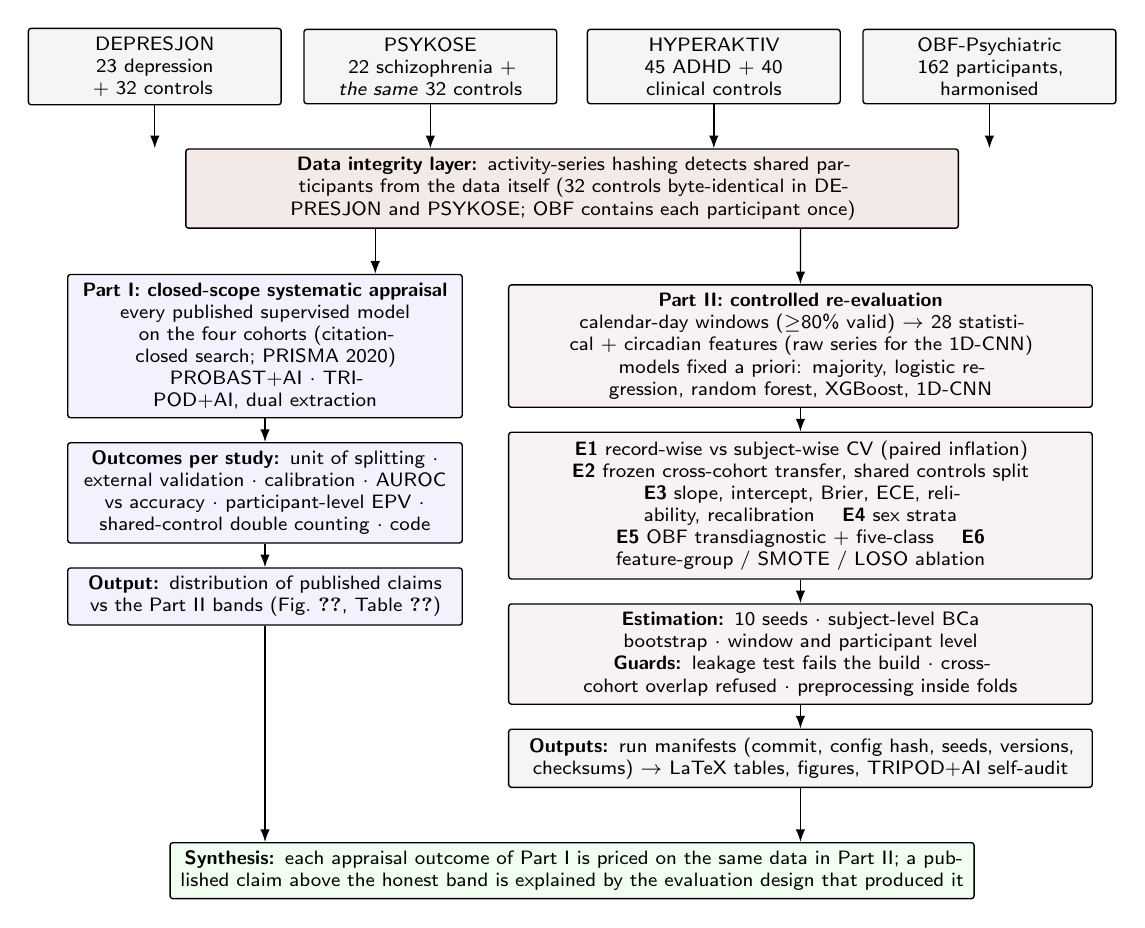
\begin{tikzpicture}[x=1cm,y=1cm,
  font=\sffamily\scriptsize,
  box/.style={draw, rounded corners=1pt, align=center, inner sep=3pt, minimum height=7mm, fill=white, line width=0.5pt},
  data/.style={box, fill=gray!8, text width=30mm},
  p1/.style={box, fill=blue!5, text width=48mm},
  p2/.style={box, fill=accent!6, text width=72mm},
  arr/.style={-{Latex[length=1.6mm]}, line width=0.5pt}]
% ----- data layer
\node[data] (dep) at (-5.3,0) {DEPRESJON\\23 depression + 32 controls};
\node[data] (psy) at (-1.8,0) {PSYKOSE\\22 schizophrenia + \emph{the same} 32 controls};
\node[data] (hyp) at (1.8,0) {HYPERAKTIV\\45 ADHD + 40 clinical controls};
\node[data] (obf) at (5.3,0) {OBF-Psychiatric\\162 participants, harmonised};
\node[box, fill=accent!10, text width=96mm] (hash) at (0,-1.55) {\textbf{Data integrity layer:} activity-series hashing detects shared participants from the data itself (32 controls byte-identical in DEPRESJON and PSYKOSE; OBF contains each participant once)};
\foreach \n in {dep,psy,hyp,obf} \draw[arr] (\n.south) -- (\n.south|-hash.north);
% ----- Part I (left column)
\node[p1] (p1a) at (-3.9,-3.55) {\textbf{Part I: closed-scope systematic appraisal}\\every published supervised model on the four cohorts (citation-closed search; PRISMA 2020)\\PROBAST+AI $\cdot$ TRIPOD+AI, dual extraction};
\node[p1, below=3mm of p1a] (p1b) {\textbf{Outcomes per study:} unit of splitting $\cdot$ external validation $\cdot$ calibration $\cdot$ AUROC vs accuracy $\cdot$ participant-level EPV $\cdot$ shared-control double counting $\cdot$ code};
\node[p1, below=3mm of p1b] (p1c) {\textbf{Output:} distribution of published claims vs the Part II bands (Fig.~\ref{fig:part1}, Table~\ref{tab:sota})};
% ----- Part II (right column)
\node[p2] (p2a) at (2.9,-3.55) {\textbf{Part II: controlled re-evaluation}\\calendar-day windows ($\geq$80\% valid) $\rightarrow$ 28 statistical + circadian features (raw series for the 1D-CNN)\\models fixed a priori: majority, logistic regression, random forest, XGBoost, 1D-CNN};
\node[p2, below=3mm of p2a] (p2b) {\textbf{E1} record-wise vs subject-wise CV (paired inflation) \quad \textbf{E2} frozen cross-cohort transfer, shared controls split\\\textbf{E3} slope, intercept, Brier, ECE, reliability, recalibration \quad \textbf{E4} sex strata\\\textbf{E5} OBF transdiagnostic + five-class \quad \textbf{E6} feature-group / SMOTE / LOSO ablation};
\node[p2, below=3mm of p2b] (p2c) {\textbf{Estimation:} 10 seeds $\cdot$ subject-level BCa bootstrap $\cdot$ window and participant level\\\textbf{Guards:} leakage test fails the build $\cdot$ cross-cohort overlap refused $\cdot$ preprocessing inside folds};
\node[p2, below=3mm of p2c, fill=gray!8] (p2d) {\textbf{Outputs:} run manifests (commit, config hash, seeds, versions, checksums) $\rightarrow$ LaTeX tables, figures, TRIPOD+AI self-audit};
\draw[arr] ([xshift=-2.5cm]hash.south) -- ([xshift=-2.5cm]hash.south|-p1a.north);
\draw[arr] ([xshift=2.9cm]hash.south) -- (p2a.north);
\draw[arr] (p1a) -- (p1b); \draw[arr] (p1b) -- (p1c);
\draw[arr] (p2a) -- (p2b); \draw[arr] (p2b) -- (p2c); \draw[arr] (p2c) -- (p2d);
% ----- synthesis
\node[box, fill=green!6, text width=100mm] (syn) at ($(p2d.south)+(-2.9,-1.05)$) {\textbf{Synthesis:} each appraisal outcome of Part I is priced on the same data in Part II; a published claim above the honest band is explained by the evaluation design that produced it};
\draw[arr] (p1c.south) -- (p1c.south|-syn.north);
\draw[arr] (p2d.south) -- (p2d.south|-syn.north);
\end{tikzpicture}
\caption{Architecture of the study. Four open actigraphy cohorts pass through a data-level integrity check (participant hashing) into a closed-scope systematic appraisal of the published models (Part I) and a controlled re-evaluation under the designs the appraisal scores (Part II); the synthesis maps every appraisal outcome to a measured cost.}\label{fig:framework}
\end{figure}


\section{Part I: systematic appraisal of the published models}\label{sec:part1}
\subsection{Design}
Part~I is a closed-scope systematic appraisal reported following PRISMA 2020 principles; it was
not prospectively registered, and the Part~II analysis plan is fixed in versioned configuration
files in the repository. \emph{Eligibility}: peer-reviewed articles, indexed conference papers and preprints
(January 2018 to September 2026, English) that train or evaluate a supervised model to predict group
membership, symptom score or state from DEPRESJON, PSYKOSE, HYPERAKTIV or OBF-Psychiatric activity
data and report at least one performance metric; excluded are reviews, dataset descriptors without
a model, and unsupervised or purely descriptive analyses. \emph{Identification}: forward citation tracing of
the four dataset papers and searches for the dataset names (``Depresjon'', ``Psykose'',
``Hyperaktiv'', ``OBF-Psychiatric'') in Google Scholar, Semantic Scholar, PubMed/PMC, arXiv and the
publishers' sites, run in September 2026 (Supplementary Table S3 records sources and dates).
\emph{Screening and extraction}: titles, abstracts and, where accessible, full texts were
screened and extracted by the authors against a fixed codebook; extractions that could rest only
on the abstract and metadata are marked as such in Table~\ref{tab:part1} and treated as a
limitation.
\emph{Appraisal}: PROBAST+AI (four domains) and the 27-item TRIPOD+AI checklist in duplicate.
\emph{Pre-specified outcomes per study}: unit of splitting (participant, day/window, unstated);
any external validation; calibration reported; AUROC reported or accuracy only; participant-level
events per candidate predictor; use of both DEPRESJON and PSYKOSE and, if so, recognition of the
shared control group; code availability; and the best reported performance, so that claims can be
plotted against the Part~II bands.

\subsection{Results of Part I}
Twenty-eight eligible studies were identified (Table~\ref{tab:part1}; sources in Supplementary
Table S4): 13 on DEPRESJON alone, 3 on PSYKOSE alone, 6 on HYPERAKTIV, 2 on OBF-Psychiatric and
4 combining DEPRESJON with PSYKOSE. Seven split by participant (the four dataset papers and three
follow-ups), 9 split by day or window, and 12 did not state the unit in the available text. None
reported any calibration measure. None validated a model on a second cohort; one preprint claims
an independent set under a ``modified leave-one-out'' scheme. Four released code, all of them
dataset papers. Every study reporting accuracy above 0.85 on DEPRESJON or above 0.90 on PSYKOSE
used, or did not state, a day-level unit (Figure~\ref{fig:part1}). Of the four studies that
combined DEPRESJON and PSYKOSE, the OBF-Psychiatric descriptor lists the shared controls once by
construction; none of the other three states how the shared control group was handled.
Participant-level events per candidate predictor cannot exceed 23 cases divided by the number of
candidate predictors on DEPRESJON and 22 on PSYKOSE, i.e.\ below 1 for any feature set larger
than the number of cases, and no study reported the quantity.

% Auto-generated by scripts/part1_figure.py from part1_studies.csv
\begin{table}[!htbp]\centering\caption{Part I: eligible published supervised models on the four cohorts (sources in Supplementary Table S4). $^{a}$Extracted from the abstract and metadata (full text not accessible at extraction); n.r.\ = not reported there. Split unit: participant = leave-one-participant-out or grouped folds; day/window = folds over days or windows; unstated = not stated in the available text.}\label{tab:part1}\scriptsize
\begin{adjustbox}{max width=\linewidth}\begin{tabular}{llllllllll}\toprule
ID & First author & Year & Cohorts & Best model & Split unit & Best reported & Calib. & Ext. val. & Code\\\midrule
S01 & Garcia-Ceja & 2018 & DEPRESJON & Random forest / DNN & participant (leave-one-patient-out) & F1 0.73 & no & no & yes\\
S02$^{a}$ & Zanella-Calzada & 2019 & DEPRESJON & Random forest & day/window & accuracy 0.89 & no & no & no\\
S03$^{a}$ & Frogner & 2019 & DEPRESJON & 1D-CNN & participant (leave-one-participant-out) & F1 n.r. & no & no & no\\
S04$^{a}$ & Jakobsen & 2020 & DEPRESJON & Random forest / DNN / CNN & participant (leave-one-out) & accuracy n.r. & no & no & no\\
S05 & Jakobsen & 2020 & PSYKOSE & Classical ML & participant (leave-one-patient-out) & F1 n.r. & no & no & yes\\
S06 & Hicks & 2021 & HYPERAKTIV & Classical ML & unstated (10-fold on features) & accuracy n.r. & no & no & yes\\
S07$^{a}$ & Rodriguez-Ruiz & 2022 & DEPRESJON & 2D-CNN & day/window & accuracy 0.767 & no & no & no\\
S08$^{a}$ & Rodriguez-Ruiz & 2022 & DEPRESJON+PSYKOSE & CNN & day/window & accuracy n.r. & no & no & no\\
S09$^{a}$ & Kumar & 2022 & DEPRESJON & ML on autoregressive features & unstated & accuracy 0.78 & no & no & no\\
S10$^{a}$ & Ahmed (arXiv) & 2023 & DEPRESJON & Transfer learning ensemble & modified leave-one-out & accuracy 0.96 & no & claims independent set & no\\
S11$^{a}$ & Hybrid RF-ANN (arXiv) & 2023 & DEPRESJON & RF-ANN ensemble & unstated & accuracy n.r. & no & no & no\\
S12$^{a}$ & UMAP study & 2023 & DEPRESJON & ML + UMAP & unstated & accuracy n.r. & no & no & no\\
S13$^{a}$ & Genetic-algorithm feature selection & 2023 & DEPRESJON & GA feature selection + classifier & day/window (intervals) & accuracy n.r. & no & no & no\\
S14$^{a}$ & Attention CNN (IoMT) & 2023 & PSYKOSE & Deep CNN + attention & day/window & accuracy n.r. & no & no & no\\
S15$^{a}$ & Multi-branch DL & 2024 & PSYKOSE & Multi-branch deep network & day/window & accuracy 0.92 & no & no & no\\
S16$^{a}$ & DL + XAI & 2024 & PSYKOSE (+DEPRESJON) & Deep network + XAI & day/window (24-h segments) & accuracy 0.94 & no & no & no\\
S17$^{a}$ & Hopping-mean augmentation & 2024 & DEPRESJON & Augmented ML & day/window & accuracy n.r. & no & no & no\\
S18$^{a}$ & IoMT dimensionality reduction & 2024 & HYPERAKTIV & 10 classifiers on reduced features & unstated & accuracy n.r. & no & no & no\\
S19$^{a}$ & Explainable XGBoost & 2025 & DEPRESJON & XGBoost + ADASYN & unstated in abstract & accuracy 0.849 & no & no & no\\
S20$^{a}$ & Improved CNN framework & 2025 & DEPRESJON+PSYKOSE & Improved CNN & day/window & accuracy n.r. & no & no & no\\
S21$^{a}$ & Enhanced ADHD ML & 2025 & HYPERAKTIV/OBF (45 participants) & SVM & unstated & F1 0.779 & no & no & no\\
S22$^{a}$ & HYPERAKTIV ML study & 2025 & HYPERAKTIV & RF / LightGBM / SVM & unstated & accuracy n.r. & no & no & no\\
S23$^{a}$ & Multimodal digital biomarkers & 2025 & HYPERAKTIV & Bernoulli NB (actigraphy+HRV) & unstated & F1 0.79 & no & no & no\\
S24 & OBF-Psychiatric descriptor & 2025 & OBF-Psychiatric & Classical ML baselines & participant & accuracy n.r. & no & no & yes\\
S25$^{a}$ & Data-uncertainty case study & 2025 & OBF-Psychiatric (ADHD) & QC + ML & participant & nan no difference after QC & no & no & no\\
S26$^{a}$ & ViT / CoAtNet on images & 2025 & DEPRESJON+PSYKOSE & CoAtNet-Tiny & participant (three-fold subject-wise) & accuracy n.r. & no & no & no\\
S27$^{a}$ & Time-segmentation evaluation & 2026 & DEPRESJON & ML on day segments & n.r. & accuracy n.r. & no & no & no\\
S28$^{a}$ & Accurate ADHD identification & 2022 & HYPERAKTIV & ML on real-time activity & unstated & accuracy n.r. & no & no & no\\
\bottomrule\end{tabular}\end{adjustbox}\end{table}

\begin{figure}[!htbp]\centering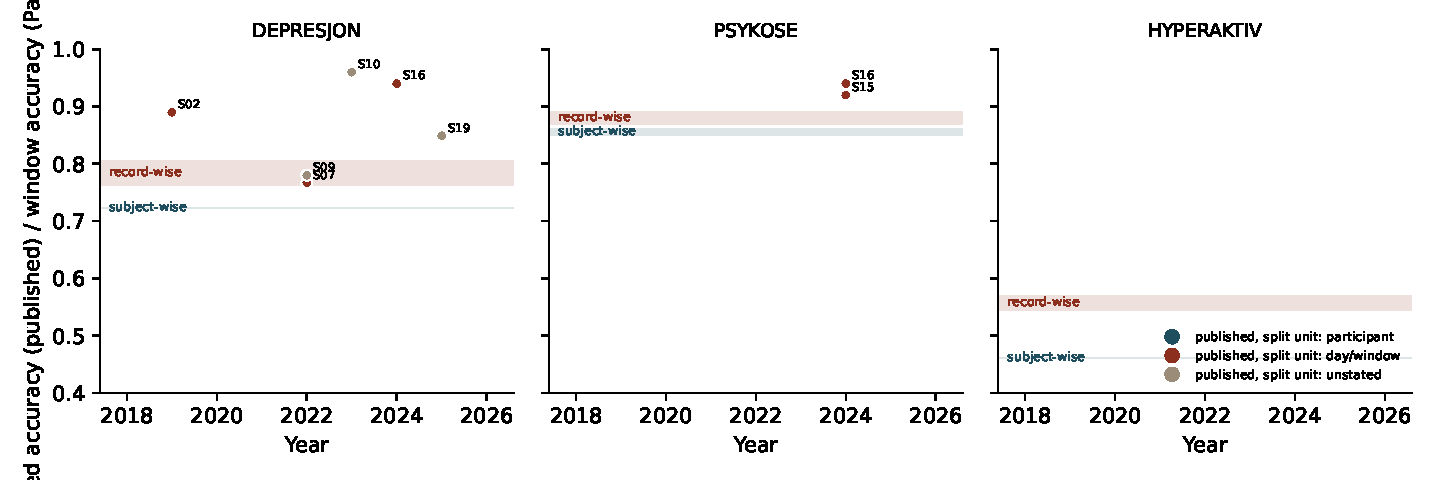
\includegraphics[width=\linewidth]{part1_claims_vs_bands.pdf}
\caption{Published best accuracies (points, labelled by study ID in Table~\ref{tab:part1}, coloured
by the unit of splitting) against the window-level accuracy bands measured in Part~II under
subject-wise and record-wise cross-validation (shaded; range over logistic regression, random
forest and XGBoost). Studies whose best metric is not accuracy, or whose value awaits full-text
verification, are not plotted.}\label{fig:part1}\end{figure}

\subsection{Conclusion of Part I}
The published literature on these cohorts reports discrimination that, where it exceeds the
dataset authors' baselines, coincides with day-level or unstated splitting (21 of 28 studies,
75\%, Wilson 95\% CI 57 to 87\%); it does not report calibration (0 of 28, 0 to 12\%); it does
not test transfer between cohorts (0 of 28); and it rarely releases code (4 of 28, 14\%, 6 to
31\%). Under PROBAST+AI these are high-risk judgements in the analysis domain, through the
signalling questions on optimism and data leakage, on evaluation of calibration as well as
discrimination, and on sample size relative to the number of candidate predictors; under
TRIPOD+AI they correspond to absent reporting of the internal-validation design, of calibration
performance, of the sample-size rationale and of code availability. The appraisal is descriptive
by construction: it establishes which practices are prevalent, not how much they matter. Part~II
measures that on the same data.

\section{Part II: controlled re-evaluation}
\subsection{Rationale and design principles}
Part~II is designed so that each of the appraisal outcomes in Part~I corresponds to one
controlled contrast on the same data, and so that the contrast cannot be attributed to anything
other than the practice under study. Four principles follow. First, \emph{models are fixed a
priori}: the same four estimators with the same hyper-parameters are used in every experiment,
so that a difference between two arms is a difference in evaluation design rather than in
model selection. Second, \emph{the unit of inference is the participant}: every split, every
bootstrap resample and every aggregate is keyed on participant identity, and window-level
numbers are reported only because they are the numbers the literature reports. Third,
\emph{integrity is enforced by code rather than by discipline}: a test fails the build if any
experiment other than E1 or E5 requests record-wise splitting, the cross-validation runner
asserts fold disjointness at run time, the external-validation runner refuses any cohort pair
with a participant on both sides, and all preprocessing lives inside a pipeline fitted on the
training fold. Fourth, \emph{every number is traceable}: each run writes a manifest with the
git commit, configuration hash, seeds, package versions and dataset checksums, and every table
and figure in this paper is written by the code from those runs.

\subsection{Data, participants and windows}
% Auto-generated by mlmh.reporting.tables -- do not edit by hand.
\begin{table}[!htbp]
\centering
\caption{Participant characteristics per cohort. HYPERAKTIV controls are psychiatric patients without ADHD (clinical controls); DEPRESJON and PSYKOSE share the same 32 healthy controls. Sex, age band and recording days from the harmonised OBF-Psychiatric metadata; day-windows are the analysis units after the 80\% validity threshold.}
\label{tab:cohorts}
\footnotesize
\begin{adjustbox}{max width=\linewidth}
\begin{tabular}{llrlllrl}
\toprule
Cohort & Group & n & Female, n (\%) & Age (modal band) & Recording days, median (range) & Valid day-windows & Clinical scale, median (IQR) \\
\midrule
depresjon & cases (depression) & 23 & 10 (43) & 45-49 & 13 (5-18) & 405 & MADRS 24 (IQR 18-26) \\
depresjon & controls (healthy\_control) & 32 & 20 (62) & 50-54 & 13 (8-20) & 739 & -- \\
psykose & cases (schizophrenia) & 22 & 3 (14) & 35-39 & 13 (12-14) & 390 & BPRS 51 (IQR 44-58) \\
psykose & controls (healthy\_control) & 32 & 20 (62) & 50-54 & 13 (8-20) & 739 & -- \\
hyperaktiv & cases (adhd) & 45 & 21 (47) & 30-39 & 7 (2-10) & 343 & ASRS 49 (IQR 40-55) \\
hyperaktiv & controls (clinical\_control) & 40 & 20 (50) & 17-29 & 7 (6-10) & 329 & ASRS 34 (IQR 25-43) \\
obf\_psychiatric & cases (adhd, clinical, depression, schizophrenia) & 130 & 54 (42) & 30-39 & 7 (2-18) & 1467 & -- \\
obf\_psychiatric & controls (control) & 32 & 20 (62) & 50-54 & 13 (8-20) & 739 & -- \\
\bottomrule
\end{tabular}
\end{adjustbox}
\end{table}

DEPRESJON \cite{garciaceja2018} comprises 23 patients with unipolar or bipolar depression
(MADRS at the start of recording, median 24, interquartile range 18 to 26) and 32 healthy
controls; PSYKOSE \cite{jakobsen2020} comprises 22 inpatients with schizophrenia (BPRS median
51, 44 to 58) and the same 32 controls; HYPERAKTIV \cite{hicks2021} comprises adults referred
for ADHD assessment, of whom 45 with ADHD and 40 clinical controls (psychiatric outpatients
without ADHD) have activity recordings, read here from the OBF-Psychiatric release
\cite{obf2025}. All cohorts were recorded with an Actiwatch (Cambridge Neurotechnology) at
one-minute resolution; recruitment, consent and clinical assessment are described in the
source publications. Table~\ref{tab:cohorts} summarises the analysed participants; sex, age
band and recording days are taken from the harmonised OBF metadata and matched to the
original cohorts by activity-series hash.

Hashing each participant's activity series confirmed two facts that the documentation states
but the literature rarely acts on: the 32 PSYKOSE control recordings are byte-identical to the
32 DEPRESJON control recordings, and OBF-Psychiatric contains each of the 162 participants
exactly once ($23 + 22 + 85 + 32$). The analysis unit was one calendar day (00:00 to 23:59) with
at least 80\% valid minutes; partial first and last days were dropped. DEPRESJON yielded
1{,}034 valid days (median 15 per participant), PSYKOSE 1{,}021 (16) and HYPERAKTIV 502 (6),
1{,}818 unique days in total; no participant lost all days. Labels are participant-level
diagnostic groups inherited by every window, and the data schema rejects a participant carrying
two labels.

\subsection{Predictors}
Twenty-eight predictors were computed per day (Supplementary Table S2), chosen to cover the
constructs the actigraphy literature associates with mood and psychotic disorders rather than to
maximise discrimination: distributional statistics of the minute counts (mean, SD, coefficient
of variation, median, 10th and 90th percentiles, maximum, skewness, kurtosis, proportion of
zero-count minutes, mean and SD of $\log(1+x)$); day/night contrasts (means for 08:00 to 22:00
and for the night, their ratio, night-time inactivity); non-parametric circadian measures on the
hourly profile (M10, L5, relative amplitude, intradaily variability, sine and cosine of the
M10-onset hour); autocorrelation at 5 and 60 minutes; spectral summaries (mean log power, dominant
within-day period); the number of rest/activity transitions; and the missing-minute fraction. No
demographic variable was used, so that the cross-cohort comparison in E2 is a comparison of
populations and not of covariate availability. A raw representation, the $\log(1+x)$-transformed
1440-minute series, feeds a one-dimensional convolutional network in a supplementary arm.

\subsection{Models and preprocessing}
Four estimators were fixed before any result was seen: a majority-class baseline (constant
prediction at the training prevalence); $L_2$-regularised logistic regression ($C=1$, class-balanced
weights); a random forest (500 trees, minimum leaf size 2, balanced subsampling); and XGBoost (300
rounds, maximum depth 3, learning rate 0.05, row and column subsampling 0.8). The two simplest
exist so that the flexible ones must earn their complexity. Hyper-parameters are library defaults
or conservative values and were not tuned, because tuning inside subject-wise folds would raise
honest performance somewhat without altering the paired inflation that E1 estimates, while
tuning inside record-wise folds would inflate it further. Median imputation and standardisation
are fitted on the training fold only, inside an \texttt{imblearn} pipeline whose sampler steps run
only at training time; no resampling was used in the main runs (E6 tests SMOTE inside folds). The
supplementary 1D-CNN has three convolution--pooling blocks, global average pooling and a linear
head, trained for a fixed 30 epochs with a class-weighted loss; it has no early stopping on the
test fold.

\subsection{Performance measures and estimation}
Discrimination is reported as AUROC (primary), accuracy, balanced accuracy, macro-F1 and
Matthews correlation at a 0.5 threshold, and area under the precision--recall curve. Calibration
is reported as the Brier score, the calibration slope (coefficient of the logit of the predicted
probability in a logistic regression of the outcome) and the calibration intercept (fitted with
the slope fixed at one) \cite{vancalster2019}, the expected calibration error over ten equal-width
bins, and reliability curves. All measures are computed at two levels: the \emph{window} level,
on every day's prediction, and the \emph{participant} level, on the mean predicted probability
per participant, which is the quantity a screening decision would use. Every experiment is
repeated over ten seeds that govern fold assignment and model randomness. Point estimates are
computed on the seed-averaged out-of-fold predictions (an ensemble over seeds; the per-seed mean
and SD are also reported), and 95\% intervals are bias-corrected and accelerated bootstrap
intervals from 1{,}000 resamples of \emph{participants}, drawing all of a participant's windows
together and using a leave-one-participant-out jackknife for the acceleration term. Resampling
windows instead of participants would treat correlated observations as independent and produce
intervals that are far too narrow. Participant-level events per predictor (EPV) are reported as
the minority-class participants divided by 28.

\subsection{Experiments}
\paragraph{E1: the cost of leaky splitting.} Five-fold cross-validation was run under two
splitters on identical data and seeds. The \emph{subject-wise} splitter is a stratified group
$k$-fold in which no participant appears on both sides of any fold. The \emph{record-wise}
splitter is a stratified $k$-fold over days that ignores participant identity, so that days from
one participant appear in training and test. The estimand is the paired difference in AUROC
(record-wise minus subject-wise) for the same participants, bootstrapped by resampling
participants in both arms simultaneously. This is the design most day-level papers on these
cohorts use; the experiment measures its optimism directly rather than inferring it.
\paragraph{E2: the cost of skipping external validation.} For each ordered cohort pair, the
model was fitted on all windows of cohort A and applied, frozen, to cohort B; the internal
comparator is subject-wise cross-validation on A. Because DEPRESJON and PSYKOSE share their
controls, each shared control was assigned at random (seed 0) to exactly one cohort, 16 to each,
so that both cohorts retain both classes and no participant crosses; the assignment table is in
the repository. Two pairs are informative (DEPRESJON $\leftrightarrow$ PSYKOSE: same controls,
different patient group, same device); the third, DEPRESJON $\rightarrow$ HYPERAKTIV, is a
deliberate label-shift control in which a depression-versus-healthy model is applied to
ADHD-versus-clinical-control data and is expected to fail.
\paragraph{E3: the calibration blind spot.} For every model in E1 (subject-wise arm) and E2, the
calibration measures above were computed, and a logistic recalibration (slope and intercept)
fitted on the training cohort's out-of-fold predictions was applied to the external predictions,
to test whether external miscalibration is repairable without access to the target cohort.
\paragraph{E4: sex strata.} Subject-wise E1 predictions were stratified by sex and the measures
recomputed with participant-level intervals; strata with fewer than six participants or one
class are omitted.
\paragraph{E5: OBF-Psychiatric.} On the harmonised release, with its single de-duplicated control
group, two tasks were evaluated under both splitters: any psychiatric group versus healthy
control (130 versus 32 participants), and the five diagnostic groups (macro one-versus-rest AUROC).
\paragraph{E6: ablation.} Under subject-wise cross-validation, with logistic regression and
XGBoost and five seeds: each feature group dropped and each used alone (distributional,
day/night, circadian, temporal/spectral); SMOTE applied inside training folds; and
leave-one-subject-out in place of five-fold. E6 answers the objection that honest performance
is low only because the feature set, the class balance or the fold count was unfavourable.

\subsection{E1 results: the cost of leaky splitting}
% Auto-generated by mlmh.reporting.tables -- do not edit by hand.
\begin{table}[!htbp]
\centering
\caption{E1, window-level AUROC under subject-wise versus record-wise five-fold cross-validation. Estimates on seed-averaged out-of-fold predictions with subject-level BCa 95\% bootstrap intervals; inflation is the paired record-wise minus subject-wise difference.}
\label{tab:e1}
\footnotesize
\begin{adjustbox}{max width=\linewidth}
\begin{tabular}{llccc}
\toprule
Cohort & Model & AUROC subject-wise & AUROC record-wise & Inflation (paired) \\
\midrule
depresjon & Majority class & 0.465 [0.292, 0.653] & 0.491 [0.459, 0.528] & 0.026 [-0.147, 0.218] \\
depresjon & Logistic regression & 0.779 [0.675, 0.861] & 0.845 [0.781, 0.896] & 0.065 [0.024, 0.122] \\
depresjon & Random forest & 0.770 [0.681, 0.848] & 0.877 [0.823, 0.923] & 0.107 [0.058, 0.168] \\
depresjon & XGBoost & 0.764 [0.675, 0.842] & 0.878 [0.830, 0.918] & 0.114 [0.060, 0.181] \\
psykose & Majority class & 0.437 [0.267, 0.632] & 0.500 [0.470, 0.535] & 0.062 [-0.113, 0.241] \\
psykose & Logistic regression & 0.907 [0.820, 0.942] & 0.927 [0.875, 0.955] & 0.020 [0.006, 0.041] \\
psykose & Random forest & 0.893 [0.798, 0.934] & 0.937 [0.890, 0.962] & 0.044 [0.017, 0.080] \\
psykose & XGBoost & 0.903 [0.810, 0.941] & 0.945 [0.907, 0.969] & 0.042 [0.016, 0.078] \\
hyperaktiv & Majority class & 0.493 [0.355, 0.628] & 0.483 [0.433, 0.533] & -0.010 [-0.170, 0.148] \\
hyperaktiv & Logistic regression & 0.449 [0.360, 0.535] & 0.579 [0.486, 0.661] & 0.130 [0.095, 0.167] \\
hyperaktiv & Random forest & 0.443 [0.361, 0.534] & 0.612 [0.526, 0.692] & 0.169 [0.135, 0.206] \\
hyperaktiv & XGBoost & 0.442 [0.360, 0.524] & 0.593 [0.518, 0.664] & 0.151 [0.116, 0.186] \\
\bottomrule
\end{tabular}
\end{adjustbox}
\end{table}

% Auto-generated by mlmh.reporting.tables -- do not edit by hand.
\begin{table}[!htbp]
\centering
\caption{E1, participant-level AUROC under subject-wise versus record-wise five-fold cross-validation. Estimates on seed-averaged out-of-fold predictions with subject-level BCa 95\% bootstrap intervals; inflation is the paired record-wise minus subject-wise difference.}
\label{tab:e1subj}
\footnotesize
\begin{adjustbox}{max width=\linewidth}
\begin{tabular}{llccc}
\toprule
Cohort & Model & AUROC subject-wise & AUROC record-wise & Inflation (paired) \\
\midrule
depresjon & Majority class & 0.423 [0.300, 0.551] & 0.427 [0.295, 0.555] & 0.001 [-0.191, 0.202] \\
depresjon & Logistic regression & 0.899 [0.822, 0.969] & 0.965 [0.927, 0.990] & 0.065 [0.011, 0.109] \\
depresjon & Random forest & 0.883 [0.812, 0.948] & 0.977 [0.949, 1.000] & 0.094 [0.041, 0.146] \\
depresjon & XGBoost & 0.874 [0.795, 0.947] & 0.985 [0.964, 1.000] & 0.111 [0.040, 0.175] \\
psykose & Majority class & 0.419 [0.278, 0.557] & 0.462 [0.331, 0.593] & 0.043 [-0.148, 0.227] \\
psykose & Logistic regression & 0.974 [0.943, 1.000] & 0.994 [0.983, 1.000] & 0.020 [0.000, 0.043] \\
psykose & Random forest & 0.956 [0.913, 0.997] & 0.994 [0.983, 1.000] & 0.038 [0.000, 0.074] \\
psykose & XGBoost & 0.969 [0.935, 1.000] & 0.997 [0.991, 1.000] & 0.028 [0.000, 0.059] \\
hyperaktiv & Majority class & 0.497 [0.398, 0.597] & 0.443 [0.349, 0.540] & -0.054 [-0.203, 0.106] \\
hyperaktiv & Logistic regression & 0.424 [0.328, 0.519] & 0.601 [0.502, 0.695] & 0.177 [0.131, 0.221] \\
hyperaktiv & Random forest & 0.424 [0.333, 0.518] & 0.641 [0.550, 0.722] & 0.217 [0.177, 0.257] \\
hyperaktiv & XGBoost & 0.438 [0.337, 0.530] & 0.652 [0.555, 0.732] & 0.214 [0.173, 0.261] \\
\bottomrule
\end{tabular}
\end{adjustbox}
\end{table}

\begin{figure}[!htbp]\centering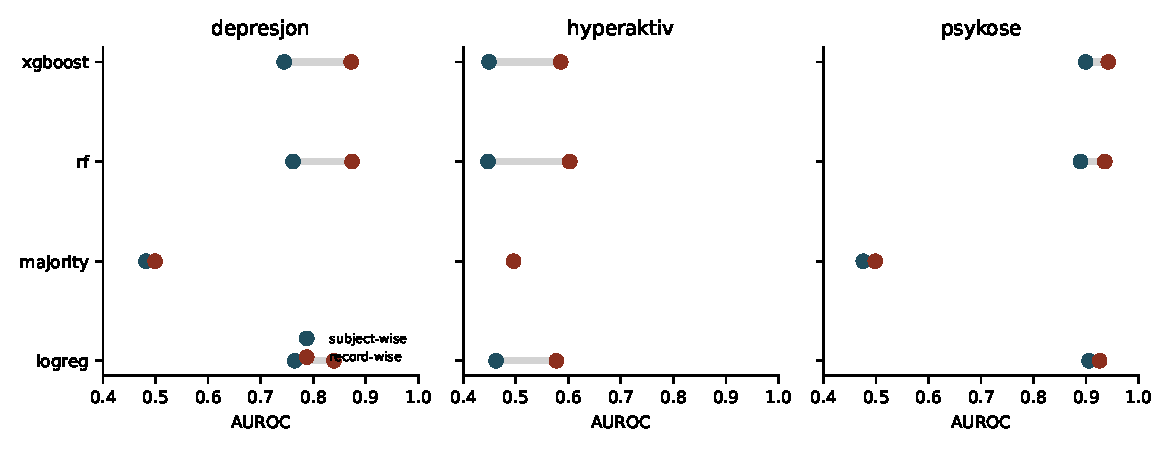
\includegraphics[width=\linewidth]{e1_inflation_auroc.pdf}
\caption{E1. Window-level AUROC of each model under subject-wise (dark) and record-wise (red) five-fold cross-validation; the grey bar is the leakage inflation.}\label{fig:e1}\end{figure}
Record-wise splitting raised AUROC for every informative model in every cohort, at both levels
(Tables~\ref{tab:e1} and~\ref{tab:e1subj}, Figure~\ref{fig:e1}). On DEPRESJON, XGBoost rose from
0.764 (95\% CI 0.675 to 0.842) to 0.878 (0.830 to 0.918) at window level, a paired inflation of
0.114 (0.060 to 0.181); at participant level the honest 0.874 became 0.985, and random forest and
logistic regression showed the same pattern with inflations of 0.107 and 0.065. On PSYKOSE, where
schizophrenia produces a large and consistent activity deficit and honest discrimination is
already 0.893 to 0.907, the inflation was smaller (0.020 to 0.044) but still excluded zero, and
the participant-level leaky estimates were 0.994 to 0.997. On HYPERAKTIV the honest estimate was
at or below chance for every model (0.442 to 0.449 at window level, 0.424 to 0.438 at
participant level), consistent with a recent report that quality-controlled OBF activity features
do not separate ADHD from controls \cite{obf2025}; record-wise splitting nevertheless produced
0.579 to 0.612 at window level and 0.601 to 0.652 at participant level, an inflation of 0.130 to
0.169 with intervals excluding zero. Leakage did not merely exaggerate a real signal; it created
one. Across cohorts the ordering was stable: logistic regression inflated least (0.065, 0.020,
0.130) and the tree ensembles most (up to 0.114, 0.044, 0.169), as expected if the mechanism is
memorisation of participant-specific activity signatures. Accuracy and macro-F1 behaved
identically (Table~\ref{tab:e1full}).

The 1D-CNN on the raw series did not earn its complexity. Under subject-wise splitting its
seed-averaged AUROC was 0.696 (0.576 to 0.795) on DEPRESJON, 0.849 (0.744 to 0.910) on PSYKOSE and
0.459 (0.356 to 0.588) on HYPERAKTIV, below the feature-based models in every cohort, and it was
unstable across seeds (per-seed means 0.61, 0.74 and 0.48). Its window-level inflation under
record-wise splitting was small, but its participant-level estimate rose from 0.738 to 0.912 on
DEPRESJON and from 0.922 to 0.986 on PSYKOSE (Tables~\ref{tab:e1_e1_cnn} and
\ref{tab:e1subj_e1_cnn}): the network learned to recognise participants across days.
% Auto-generated by mlmh.reporting.tables -- do not edit by hand.
\begin{table}[!htbp]
\centering
\caption{E1: window-level discrimination and calibration for every model, cohort and splitting design (per-seed means over ten seeds).}
\label{tab:e1full}
\footnotesize
\begin{adjustbox}{max width=\linewidth}
\begin{tabular}{llllllllll}
\toprule
Cohort & Model & Split & Accuracy & Macro-F1 & AUROC & Brier & Cal. slope & Cal. intercept & ECE \\
\midrule
depresjon & Majority class & subject-wise & 0.653 & 0.395 & 0.482 & 0.227 & -4.01 & -0.00 & 0.000 \\
depresjon & Majority class & record-wise & 0.653 & 0.395 & 0.499 & 0.227 & 0.29 & 0.00 & 0.000 \\
depresjon & Logistic regression & subject-wise & 0.722 & 0.706 & 0.765 & 0.194 & 0.52 & -0.54 & 0.118 \\
depresjon & Logistic regression & record-wise & 0.761 & 0.750 & 0.840 & 0.163 & 0.90 & -0.62 & 0.095 \\
depresjon & Random forest & subject-wise & 0.724 & 0.679 & 0.762 & 0.185 & 0.69 & 0.01 & 0.061 \\
depresjon & Random forest & record-wise & 0.806 & 0.782 & 0.874 & 0.136 & 1.23 & -0.11 & 0.039 \\
depresjon & XGBoost & subject-wise & 0.722 & 0.676 & 0.745 & 0.202 & 0.43 & 0.29 & 0.123 \\
depresjon & XGBoost & record-wise & 0.802 & 0.776 & 0.872 & 0.137 & 0.82 & 0.07 & 0.039 \\
psykose & Majority class & subject-wise & 0.661 & 0.398 & 0.476 & 0.224 & -3.95 & 0.00 & 0.000 \\
psykose & Majority class & record-wise & 0.661 & 0.398 & 0.499 & 0.224 & 0.31 & 0.00 & 0.000 \\
psykose & Logistic regression & subject-wise & 0.856 & 0.842 & 0.906 & 0.115 & 0.90 & -0.60 & 0.086 \\
psykose & Logistic regression & record-wise & 0.868 & 0.855 & 0.926 & 0.103 & 1.07 & -0.62 & 0.078 \\
psykose & Random forest & subject-wise & 0.850 & 0.829 & 0.889 & 0.118 & 0.95 & -0.12 & 0.048 \\
psykose & Random forest & record-wise & 0.878 & 0.861 & 0.936 & 0.093 & 1.32 & -0.17 & 0.048 \\
psykose & XGBoost & subject-wise & 0.862 & 0.842 & 0.899 & 0.108 & 0.71 & 0.15 & 0.046 \\
psykose & XGBoost & record-wise & 0.891 & 0.876 & 0.942 & 0.082 & 0.91 & 0.07 & 0.026 \\
hyperaktiv & Majority class & subject-wise & 0.504 & 0.335 & 0.496 & 0.250 & 0.00 & 0.00 & 0.000 \\
hyperaktiv & Majority class & record-wise & 0.504 & 0.335 & 0.496 & 0.250 & 0.00 & 0.00 & 0.000 \\
hyperaktiv & Logistic regression & subject-wise & 0.461 & 0.460 & 0.463 & 0.286 & -0.21 & -0.01 & 0.160 \\
hyperaktiv & Logistic regression & record-wise & 0.543 & 0.543 & 0.577 & 0.252 & 0.21 & 0.01 & 0.074 \\
hyperaktiv & Random forest & subject-wise & 0.463 & 0.462 & 0.447 & 0.286 & -0.32 & 0.00 & 0.156 \\
hyperaktiv & Random forest & record-wise & 0.571 & 0.571 & 0.603 & 0.245 & 0.57 & 0.00 & 0.055 \\
hyperaktiv & XGBoost & subject-wise & 0.460 & 0.460 & 0.449 & 0.330 & -0.15 & 0.00 & 0.248 \\
hyperaktiv & XGBoost & record-wise & 0.557 & 0.557 & 0.586 & 0.271 & 0.26 & 0.00 & 0.151 \\
\bottomrule
\end{tabular}
\end{adjustbox}
\end{table}

% Auto-generated by mlmh.reporting.tables -- do not edit by hand.
\begin{table}[!htbp]
\centering
\caption{E1, window-level AUROC under subject-wise versus record-wise five-fold cross-validation. Estimates on seed-averaged out-of-fold predictions with subject-level BCa 95\% bootstrap intervals; inflation is the paired record-wise minus subject-wise difference.}
\label{tab:e1_e1_cnn}
\footnotesize
\begin{adjustbox}{max width=\linewidth}
\begin{tabular}{llccc}
\toprule
Cohort & Model & AUROC subject-wise & AUROC record-wise & Inflation (paired) \\
\midrule
depresjon & 1D-CNN & 0.696 [0.576, 0.795] & 0.729 [0.671, 0.784] & 0.033 [-0.063, 0.122] \\
psykose & 1D-CNN & 0.849 [0.744, 0.910] & 0.892 [0.836, 0.935] & 0.043 [-0.000, 0.095] \\
hyperaktiv & 1D-CNN & 0.459 [0.356, 0.588] & 0.513 [0.447, 0.578] & 0.054 [-0.079, 0.189] \\
\bottomrule
\end{tabular}
\end{adjustbox}
\end{table}
% Auto-generated by mlmh.reporting.tables -- do not edit by hand.
\begin{table}[!htbp]
\centering
\caption{E1, participant-level AUROC under subject-wise versus record-wise five-fold cross-validation. Estimates on seed-averaged out-of-fold predictions with subject-level BCa 95\% bootstrap intervals; inflation is the paired record-wise minus subject-wise difference.}
\label{tab:e1subj_e1_cnn}
\footnotesize
\begin{adjustbox}{max width=\linewidth}
\begin{tabular}{llccc}
\toprule
Cohort & Model & AUROC subject-wise & AUROC record-wise & Inflation (paired) \\
\midrule
depresjon & 1D-CNN & 0.738 [0.634, 0.844] & 0.912 [0.837, 0.959] & 0.174 [0.067, 0.270] \\
psykose & 1D-CNN & 0.922 [0.852, 0.976] & 0.986 [0.963, 1.000] & 0.064 [0.016, 0.111] \\
hyperaktiv & 1D-CNN & 0.455 [0.371, 0.563] & 0.529 [0.432, 0.622] & 0.074 [-0.060, 0.208] \\
\bottomrule
\end{tabular}
\end{adjustbox}
\end{table}


\subsection{E2 results: the cost of skipping external validation}
% Auto-generated by mlmh -- do not edit by hand.
\begin{table}[!htbp]
\centering
\caption{E2: internal (subject-wise CV on the training cohort) versus external (unchanged model applied to the second cohort) performance. Window-level estimates, mean over seeds, subject-level BCa 95\% intervals. EPV = minority-class subjects per candidate predictor in the training cohort.}
\label{tab:e2}
\footnotesize
\begin{adjustbox}{max width=\linewidth}
\begin{tabular}{llllllllll}
\toprule
Train $\rightarrow$ Test & Model & EPV & Internal AUROC & External AUROC & $\Delta$ & Int. slope & Ext. slope & Ext. intercept & Ext. Brier \\
\midrule
depresjon $\rightarrow$ psykose & Majority class & 0.6 & 0.465 [0.224, 0.662] & 0.500 [0.500, 0.500] & +0.035 & -4.16 & 0.00 & -0.02 & 0.250 \\
depresjon $\rightarrow$ psykose & Logistic regression & 0.6 & 0.779 [0.701, 0.871] & 0.779 [0.676, 0.847] & -0.000 & 0.66 & 0.50 & 0.06 & 0.193 \\
depresjon $\rightarrow$ psykose & Random forest & 0.6 & 0.770 [0.607, 0.837] & 0.776 [0.688, 0.846] & +0.006 & 0.58 & 0.80 & -0.02 & 0.193 \\
depresjon $\rightarrow$ psykose & XGBoost & 0.6 & 0.764 [0.608, 0.825] & 0.769 [0.678, 0.835] & +0.005 & 0.34 & 0.55 & -0.01 & 0.204 \\
psykose $\rightarrow$ depresjon & Majority class & 0.6 & 0.390 [0.206, 0.601] & 0.500 [0.500, 0.500] & +0.110 & -4.07 & 0.00 & 0.06 & 0.250 \\
psykose $\rightarrow$ depresjon & Logistic regression & 0.6 & 0.885 [0.790, 0.938] & 0.689 [0.564, 0.793] & -0.196 & 0.72 & 0.27 & 1.20 & 0.262 \\
psykose $\rightarrow$ depresjon & Random forest & 0.6 & 0.854 [0.756, 0.926] & 0.728 [0.620, 0.818] & -0.126 & 0.76 & 0.63 & 0.74 & 0.225 \\
psykose $\rightarrow$ depresjon & XGBoost & 0.6 & 0.877 [0.793, 0.936] & 0.671 [0.569, 0.770] & -0.206 & 0.55 & 0.30 & 1.44 & 0.285 \\
depresjon $\rightarrow$ hyperaktiv & Majority class & 0.8 & 0.465 [0.292, 0.653] & 0.500 [0.500, 0.500] & +0.035 & -4.01 & -0.01 & 0.65 & 0.275 \\
depresjon $\rightarrow$ hyperaktiv & Logistic regression & 0.8 & 0.779 [0.675, 0.861] & 0.442 [0.348, 0.532] & -0.338 & 0.52 & -0.16 & -0.42 & 0.350 \\
depresjon $\rightarrow$ hyperaktiv & Random forest & 0.8 & 0.770 [0.681, 0.848] & 0.461 [0.360, 0.557] & -0.310 & 0.69 & -0.15 & 0.33 & 0.317 \\
depresjon $\rightarrow$ hyperaktiv & XGBoost & 0.8 & 0.764 [0.675, 0.842] & 0.459 [0.358, 0.550] & -0.305 & 0.43 & -0.09 & 0.48 & 0.364 \\
\bottomrule
\end{tabular}
\end{adjustbox}
\end{table}

\begin{figure}[!htbp]\centering
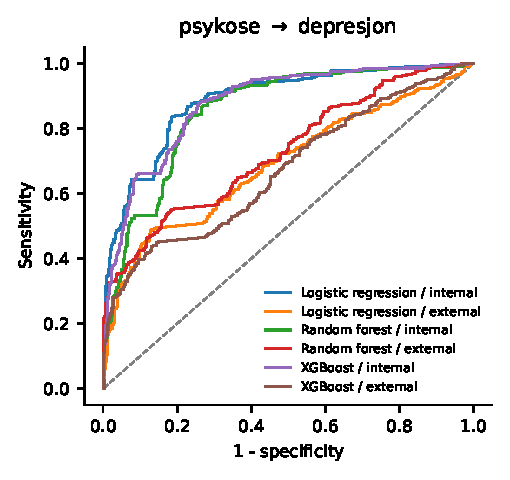
\includegraphics[width=.48\linewidth]{e2_roc_psykose_to_depresjon.pdf}\hfill
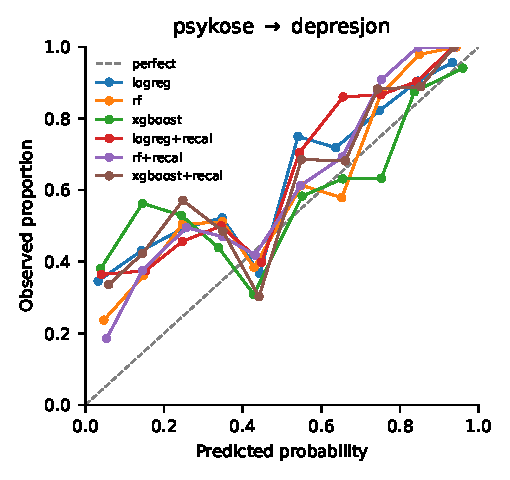
\includegraphics[width=.48\linewidth]{e3_reliability_psykose_to_depresjon.pdf}
\caption{E2/E3, PSYKOSE $\rightarrow$ DEPRESJON. Left: ROC curves of the internal (subject-wise CV on PSYKOSE) and external (frozen model on DEPRESJON) predictions. Right: reliability curves of the external predictions before and after logistic recalibration fitted on the training cohort.}\label{fig:e2}\end{figure}
Transfer was asymmetric (Table~\ref{tab:e2}). Models trained on DEPRESJON, whose positive class
is the milder activity deficit, separated schizophrenia from the held-out controls as well as
they had separated depression internally: external AUROC 0.769 to 0.779 against internal 0.764 to
0.779, with calibration slopes of 0.50 to 0.81 and intercepts near zero. Models trained on
PSYKOSE, whose positive class is the more severe deficit, lost 0.13 to 0.21 AUROC when applied to
DEPRESJON (logistic regression 0.885 $\rightarrow$ 0.689; random forest 0.854 $\rightarrow$ 0.728;
XGBoost 0.877 $\rightarrow$ 0.671), and their probabilities were both overconfident and shifted:
slopes 0.27 to 0.63, intercepts 0.74 to 1.44, Brier scores 0.22 to 0.29 against 0.25 for a
constant prediction (Figure~\ref{fig:e2}). A model that had looked excellent internally would
have been worse than useless as a probability on the new cohort. The label-shift pair DEPRESJON
$\rightarrow$ HYPERAKTIV fell to AUROC 0.442 to 0.460 with negative slopes, as designed; a paper
that reported this transfer as ``external validation'' of a mental-disorder detector would be
reporting noise. Participant-level EPV in the training cohorts was 0.6 (DEPRESJON and PSYKOSE
after the control split) and 0.8 (HYPERAKTIV), one to two orders of magnitude below any
guidance, while the window-level counts (hundreds of days per class) would have suggested
adequacy.

\subsection{E3 results: the calibration blind spot}
\begin{figure}[!htbp]\centering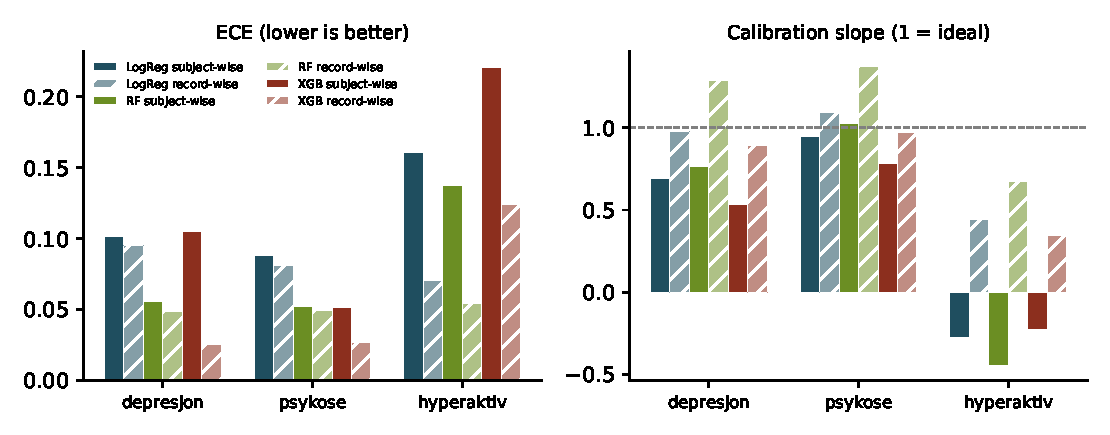
\includegraphics[width=.9\linewidth]{e3_ece_slope_comparison.pdf}
\caption{E3. Expected calibration error (left) and calibration slope (right) of every model under subject-wise (solid) and record-wise (hatched) cross-validation. Record-wise models appear better calibrated because they score participants they have seen.}\label{fig:ece}\end{figure}
\begin{figure}[!htbp]\centering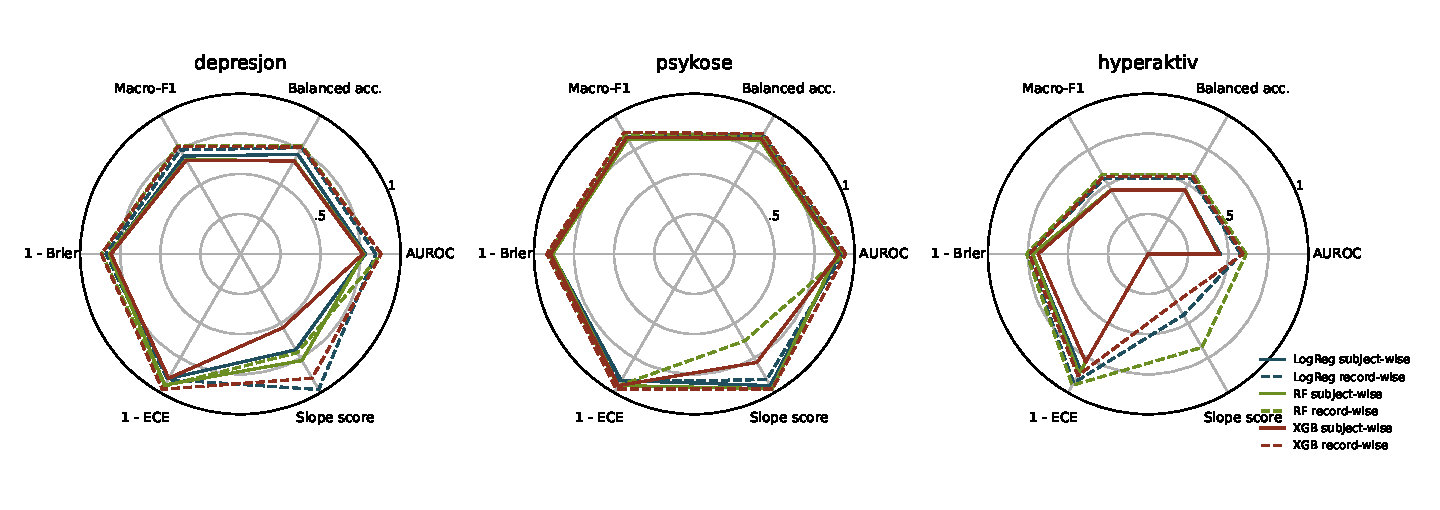
\includegraphics[width=\linewidth]{e1_radar_models.pdf}
\caption{Multi-metric profile of the models per cohort (AUROC, balanced accuracy, macro-F1, $1-$Brier, $1-$ECE and a slope score $1-|1-\text{slope}|$) under subject-wise (solid) and record-wise (dashed) cross-validation. Leakage expands every axis at once; on HYPERAKTIV the honest profile collapses to chance while the leaky profile does not.}\label{fig:radar}\end{figure}
Under honest splitting the informative models were already miscalibrated (Table~\ref{tab:e3},
Figures~\ref{fig:ece} and~\ref{fig:radar}). On DEPRESJON, slopes were 0.53 (XGBoost), 0.69
(logistic regression) and 0.77 (random forest), with ECE 0.06 to 0.11; on PSYKOSE, 0.95 for
logistic regression; on HYPERAKTIV, slopes were negative and ECE 0.14 to 0.22, i.e.\ the models
had learned nothing and yet issued confident probabilities. Under record-wise splitting the same
models appeared markedly better calibrated (slopes 0.9 to 1.3, ECE 0.02 to 0.05 on DEPRESJON and
PSYKOSE), which is not a virtue but a symptom: they were scoring participants they had seen, and
their confidence was justified only for those participants. The radar profiles make the same
point in one view: leakage expands every axis simultaneously, and on HYPERAKTIV the honest profile
collapses to the centre while the leaky profile does not. Recalibrating external predictions with
a slope and intercept fitted on the training cohort's own out-of-fold predictions repaired the
easy direction (DEPRESJON $\rightarrow$ PSYKOSE: slopes 1.05, ECE 0.04 to 0.05 for the ensembles)
but not the hard one (PSYKOSE $\rightarrow$ DEPRESJON: slopes 0.35 to 0.77, ECE 0.13 to 0.20),
because the miscalibration there is a property of the population shift and cannot be estimated
without data from the target population.
% Auto-generated by mlmh.reporting.tables -- do not edit by hand.
\begin{table}[!htbp]
\centering
\caption{E3: calibration alongside discrimination for every model in E1 (subject-wise arm) and E2, plus logistic recalibration of external predictions.}
\label{tab:e3}
\footnotesize
\begin{adjustbox}{max width=\linewidth}
\begin{tabular}{llrrrrr}
\toprule
Exp. & Run & AUROC & Brier & Cal. slope & Cal. intercept & ECE \\
\midrule
E1 & depresjon.logreg.subject\_wise & 0.779 & 0.187 & 0.69 & -0.51 & 0.102 \\
E1 & depresjon.rf.subject\_wise & 0.770 & 0.181 & 0.77 & 0.01 & 0.056 \\
E1 & depresjon.xgboost.subject\_wise & 0.764 & 0.192 & 0.53 & 0.27 & 0.105 \\
E1 & hyperaktiv.logreg.subject\_wise & 0.449 & 0.279 & -0.28 & -0.01 & 0.161 \\
E1 & hyperaktiv.rf.subject\_wise & 0.443 & 0.281 & -0.45 & 0.00 & 0.137 \\
E1 & hyperaktiv.xgboost.subject\_wise & 0.442 & 0.313 & -0.23 & 0.00 & 0.221 \\
E1 & psykose.logreg.subject\_wise & 0.907 & 0.112 & 0.95 & -0.59 & 0.088 \\
E1 & psykose.rf.subject\_wise & 0.893 & 0.115 & 1.03 & -0.12 & 0.052 \\
E1 & psykose.xgboost.subject\_wise & 0.903 & 0.103 & 0.78 & 0.14 & 0.052 \\
E2 & depresjon-to-hyperaktiv.logreg.external & 0.442 & 0.350 & -0.16 & -0.42 & 0.291 \\
E2 & depresjon-to-hyperaktiv.rf.external & 0.461 & 0.317 & -0.15 & 0.33 & 0.214 \\
E2 & depresjon-to-hyperaktiv.xgboost.external & 0.459 & 0.363 & -0.09 & 0.47 & 0.292 \\
E2 & depresjon-to-psykose.logreg.external & 0.779 & 0.193 & 0.50 & 0.06 & 0.079 \\
E2 & depresjon-to-psykose.rf.external & 0.776 & 0.193 & 0.81 & -0.02 & 0.044 \\
E2 & depresjon-to-psykose.xgboost.external & 0.769 & 0.202 & 0.56 & -0.01 & 0.085 \\
E2 & depresjon.logreg.internal & 0.779 & 0.187 & 0.69 & -0.51 & 0.102 \\
E2 & depresjon.rf.internal & 0.770 & 0.181 & 0.77 & 0.01 & 0.056 \\
E2 & depresjon.xgboost.internal & 0.764 & 0.192 & 0.53 & 0.27 & 0.105 \\
E2 & psykose-to-depresjon.logreg.external & 0.689 & 0.262 & 0.27 & 1.20 & 0.202 \\
E2 & psykose-to-depresjon.rf.external & 0.728 & 0.225 & 0.63 & 0.74 & 0.149 \\
E2 & psykose-to-depresjon.xgboost.external & 0.671 & 0.284 & 0.31 & 1.43 & 0.229 \\
E2 & psykose.logreg.internal & 0.885 & 0.137 & 0.77 & -0.10 & 0.061 \\
E2 & psykose.rf.internal & 0.854 & 0.151 & 0.82 & -0.08 & 0.055 \\
E2 & psykose.xgboost.internal & 0.877 & 0.148 & 0.62 & -0.16 & 0.083 \\
E2 & depresjon-to-hyperaktiv.logreg.external+recal & 0.442 & 0.311 & -0.23 & 0.22 & 0.223 \\
E2 & depresjon-to-hyperaktiv.rf.external+recal & 0.461 & 0.301 & -0.20 & 0.37 & 0.176 \\
E2 & depresjon-to-hyperaktiv.xgboost.external+recal & 0.459 & 0.311 & -0.17 & 0.36 & 0.194 \\
E2 & depresjon-to-psykose.logreg.external+recal & 0.779 & 0.211 & 0.72 & 0.56 & 0.139 \\
E2 & depresjon-to-psykose.rf.external+recal & 0.776 & 0.193 & 1.05 & 0.11 & 0.041 \\
E2 & depresjon-to-psykose.xgboost.external+recal & 0.769 & 0.196 & 1.05 & 0.11 & 0.052 \\
E2 & psykose-to-depresjon.logreg.external+recal & 0.689 & 0.254 & 0.35 & 0.99 & 0.185 \\
E2 & psykose-to-depresjon.rf.external+recal & 0.728 & 0.221 & 0.77 & 0.67 & 0.129 \\
E2 & psykose-to-depresjon.xgboost.external+recal & 0.671 & 0.258 & 0.49 & 0.93 & 0.200 \\
\bottomrule
\end{tabular}
\end{adjustbox}
\end{table}


\subsection{E4 and E5 results: sex strata; transdiagnostic and five-class tasks}
% Auto-generated by mlmh.reporting.tables -- do not edit by hand.
\begin{table}[!htbp]
\centering
\caption{E4: sex-stratified performance of the subject-wise E1 models (window level, subject-level bootstrap intervals). Subgroups with fewer than six participants or a single class are omitted.}
\label{tab:e4}
\footnotesize
\begin{adjustbox}{max width=\linewidth}
\begin{tabular}{lllllrrr}
\toprule
Cohort & Model & Sex & Participants (cases) & AUROC [95\textbackslash \% CI] & Brier & Cal. slope & ECE \\
\midrule
depresjon & Logistic regression & female & 30 (10) & 0.777 [0.649, 0.872] & 0.182 & 0.75 & 0.120 \\
depresjon & Logistic regression & male & 25 (13) & 0.776 [0.562, 0.882] & 0.192 & 0.62 & 0.091 \\
depresjon & Random forest & female & 30 (10) & 0.763 [0.623, 0.870] & 0.171 & 0.75 & 0.071 \\
depresjon & Random forest & male & 25 (13) & 0.777 [0.626, 0.870] & 0.193 & 0.80 & 0.070 \\
depresjon & XGBoost & female & 30 (10) & 0.755 [0.620, 0.859] & 0.183 & 0.51 & 0.109 \\
depresjon & XGBoost & male & 25 (13) & 0.772 [0.619, 0.868] & 0.203 & 0.55 & 0.120 \\
hyperaktiv & Logistic regression & female & 41 (21) & 0.479 [0.370, 0.602] & 0.275 & -0.10 & 0.152 \\
hyperaktiv & Logistic regression & male & 44 (24) & 0.424 [0.321, 0.543] & 0.283 & -0.49 & 0.168 \\
hyperaktiv & Random forest & female & 41 (21) & 0.491 [0.371, 0.611] & 0.269 & -0.10 & 0.111 \\
hyperaktiv & Random forest & male & 44 (24) & 0.398 [0.278, 0.516] & 0.291 & -0.80 & 0.160 \\
hyperaktiv & XGBoost & female & 41 (21) & 0.498 [0.385, 0.605] & 0.293 & -0.02 & 0.211 \\
hyperaktiv & XGBoost & male & 44 (24) & 0.388 [0.278, 0.505] & 0.332 & -0.44 & 0.230 \\
psykose & Logistic regression & female & 23 (3) & 0.971 [0.915, 0.998] & 0.096 & 1.58 & 0.177 \\
psykose & Logistic regression & male & 31 (19) & 0.890 [0.771, 0.933] & 0.126 & 0.83 & 0.081 \\
psykose & Random forest & female & 23 (3) & 0.966 [0.891, 0.995] & 0.075 & 1.66 & 0.147 \\
psykose & Random forest & male & 31 (19) & 0.874 [0.765, 0.930] & 0.149 & 0.90 & 0.123 \\
psykose & XGBoost & female & 23 (3) & 0.969 [0.904, 0.997] & 0.059 & 1.16 & 0.100 \\
psykose & XGBoost & male & 31 (19) & 0.884 [0.774, 0.933] & 0.140 & 0.71 & 0.121 \\
\bottomrule
\end{tabular}
\end{adjustbox}
\end{table}

% Auto-generated by mlmh.reporting.tables -- do not edit by hand.
\begin{table}[!htbp]
\centering
\caption{E5: OBF-Psychiatric (162 participants, single control group). Transdiagnostic binary arm (any psychiatric group vs healthy control; window-level AUROC with subject-level BCa intervals) and five-class arm (macro one-vs-rest AUROC), each under subject-wise and record-wise CV.}
\label{tab:e5}
\footnotesize
\begin{adjustbox}{max width=\linewidth}
\begin{tabular}{lllrrrr}
\toprule
Arm & Model & Split & AUROC / macro-AUROC & Accuracy & Macro-F1 & Cal. slope \\
\midrule
Any psychiatric vs control & Majority class & subject-wise & 0.490 [0.358, 0.614] & 0.641 & 0.391 & 0.25 \\
Any psychiatric vs control & Majority class & record-wise & 0.500 [0.470, 0.529] & 0.641 & 0.391 & 0.25 \\
Any psychiatric vs control & Logistic regression & subject-wise & 0.795 [0.745, 0.848] & 0.741 & 0.725 & 0.78 \\
Any psychiatric vs control & Logistic regression & record-wise & 0.824 [0.777, 0.867] & 0.756 & 0.742 & 0.93 \\
Any psychiatric vs control & Random forest & subject-wise & 0.781 [0.726, 0.837] & 0.739 & 0.705 & 0.75 \\
Any psychiatric vs control & Random forest & record-wise & 0.849 [0.811, 0.887] & 0.782 & 0.755 & 1.07 \\
Any psychiatric vs control & XGBoost & subject-wise & 0.776 [0.729, 0.834] & 0.734 & 0.702 & 0.63 \\
Any psychiatric vs control & XGBoost & record-wise & 0.844 [0.810, 0.885] & 0.781 & 0.755 & 0.90 \\
Five diagnostic groups & Logistic regression & subject-wise & 0.713 [0.677, 0.750] & 0.431 & 0.390 & -- \\
Five diagnostic groups & Logistic regression & record-wise & 0.770 [0.740, 0.799] & 0.484 & 0.444 & -- \\
Five diagnostic groups & Random forest & subject-wise & 0.695 [0.662, 0.735] & 0.434 & 0.350 & -- \\
Five diagnostic groups & Random forest & record-wise & 0.811 [0.786, 0.843] & 0.558 & 0.482 & -- \\
Five diagnostic groups & XGBoost & subject-wise & 0.702 [0.670, 0.743] & 0.448 & 0.355 & -- \\
Five diagnostic groups & XGBoost & record-wise & 0.808 [0.785, 0.842] & 0.558 & 0.467 & -- \\
\bottomrule
\end{tabular}
\end{adjustbox}
\end{table}

Discrimination did not differ materially by sex on DEPRESJON (AUROC 0.76 to 0.78 in both
strata) or on HYPERAKTIV (chance in both); on PSYKOSE the female stratum contains three cases and
its apparently higher AUROC (0.97) rests on them, with intervals overlapping the male stratum
(Table~\ref{tab:e4}). Calibration slopes differed between strata more than discrimination did,
which is the usual pattern when a model's probabilities are shifted for a subgroup that is
under-represented in training. On OBF-Psychiatric, separating any psychiatric group from the
healthy controls reached AUROC 0.776 to 0.795 subject-wise and 0.824 to 0.849 record-wise
(participant level 0.856 to 0.867 versus 0.899 to 0.943); the five-class task gave a macro
one-versus-rest AUROC of 0.695 to 0.713 (accuracy 0.43 to 0.45 against a 0.28 majority rate)
subject-wise and 0.770 to 0.811 (0.48 to 0.56) record-wise (Table~\ref{tab:e5}). Inflation was
again largest for the ensembles (0.106 to 0.116 in macro-AUROC) and smallest for logistic
regression (0.057). A transdiagnostic actigraphy signal exists, but it is moderate, and the
five-way separation is weak once participants are held out.

\subsection{E6 results: ablation}
% Auto-generated by mlmh.reporting.tables -- do not edit by hand.
\begin{table}[!htbp]
\centering
\caption{E6: ablation under subject-wise CV. Feature-group ablations (drop-one and only-one), SMOTE applied inside training folds, and leave-one-subject-out (LOSO) in place of five-fold CV. Window-level estimates with subject-level BCa intervals.}
\label{tab:e6}
\footnotesize
\begin{adjustbox}{max width=\linewidth}
\begin{tabular}{lllrlrrrr}
\toprule
Cohort & Model & Variant & k & AUROC [95\textbackslash \% CI] & Subject AUROC & Brier & Cal. slope & ECE \\
\midrule
depresjon & Logistic regression & all\textbackslash \_features & 28 & 0.785 [0.694, 0.853] & 0.902 & 0.187 & 0.71 & 0.103 \\
depresjon & Logistic regression & drop\textbackslash \_distributional & 16 & 0.758 [0.649, 0.837] & 0.890 & 0.198 & 0.69 & 0.119 \\
depresjon & Logistic regression & only\textbackslash \_distributional & 12 & 0.755 [0.652, 0.836] & 0.838 & 0.200 & 0.79 & 0.115 \\
depresjon & Logistic regression & drop\textbackslash \_day\textbackslash \_night & 24 & 0.781 [0.687, 0.850] & 0.893 & 0.188 & 0.74 & 0.108 \\
depresjon & Logistic regression & only\textbackslash \_day\textbackslash \_night & 4 & 0.458 [0.358, 0.541] & 0.577 & 0.257 & -0.07 & 0.149 \\
depresjon & Logistic regression & drop\textbackslash \_circadian & 22 & 0.797 [0.708, 0.863] & 0.906 & 0.181 & 0.78 & 0.103 \\
depresjon & Logistic regression & only\textbackslash \_circadian & 6 & 0.640 [0.533, 0.722] & 0.783 & 0.239 & 0.59 & 0.152 \\
depresjon & Logistic regression & drop\textbackslash \_temporal\textbackslash \_spectral & 22 & 0.771 [0.678, 0.840] & 0.890 & 0.193 & 0.73 & 0.102 \\
depresjon & Logistic regression & only\textbackslash \_temporal\textbackslash \_spectral & 6 & 0.740 [0.551, 0.829] & 0.874 & 0.211 & 0.85 & 0.178 \\
depresjon & Logistic regression & all\textbackslash \_features+smote\textbackslash \_in\textbackslash \_fold & 28 & 0.786 [0.697, 0.852] & 0.899 & 0.186 & 0.68 & 0.097 \\
depresjon & Logistic regression & all\textbackslash \_features+loso & 28 & 0.773 [0.660, 0.849] & 0.890 & 0.191 & 0.63 & 0.111 \\
depresjon & XGBoost & all\textbackslash \_features & 28 & 0.768 [0.685, 0.837] & 0.871 & 0.192 & 0.53 & 0.101 \\
depresjon & XGBoost & drop\textbackslash \_distributional & 16 & 0.788 [0.711, 0.852] & 0.905 & 0.181 & 0.59 & 0.093 \\
depresjon & XGBoost & only\textbackslash \_distributional & 12 & 0.739 [0.640, 0.812] & 0.844 & 0.196 & 0.54 & 0.090 \\
depresjon & XGBoost & drop\textbackslash \_day\textbackslash \_night & 24 & 0.769 [0.685, 0.836] & 0.878 & 0.190 & 0.53 & 0.093 \\
depresjon & XGBoost & only\textbackslash \_day\textbackslash \_night & 4 & 0.769 [0.682, 0.841] & 0.875 & 0.185 & 0.63 & 0.062 \\
depresjon & XGBoost & drop\textbackslash \_circadian & 22 & 0.787 [0.707, 0.851] & 0.912 & 0.181 & 0.58 & 0.090 \\
depresjon & XGBoost & only\textbackslash \_circadian & 6 & 0.711 [0.606, 0.796] & 0.817 & 0.203 & 0.52 & 0.090 \\
depresjon & XGBoost & drop\textbackslash \_temporal\textbackslash \_spectral & 22 & 0.740 [0.642, 0.817] & 0.825 & 0.204 & 0.49 & 0.117 \\
depresjon & XGBoost & only\textbackslash \_temporal\textbackslash \_spectral & 6 & 0.802 [0.737, 0.859] & 0.947 & 0.168 & 0.68 & 0.053 \\
depresjon & XGBoost & all\textbackslash \_features+smote\textbackslash \_in\textbackslash \_fold & 28 & 0.761 [0.676, 0.835] & 0.879 & 0.196 & 0.51 & 0.109 \\
depresjon & XGBoost & all\textbackslash \_features+loso & 28 & 0.745 [0.649, 0.820] & 0.853 & 0.205 & 0.45 & 0.124 \\
psykose & Logistic regression & all\textbackslash \_features & 28 & 0.903 [0.807, 0.937] & 0.973 & 0.115 & 0.92 & 0.090 \\
psykose & Logistic regression & drop\textbackslash \_distributional & 16 & 0.845 [0.754, 0.892] & 0.952 & 0.159 & 0.87 & 0.119 \\
psykose & Logistic regression & only\textbackslash \_distributional & 12 & 0.875 [0.785, 0.921] & 0.945 & 0.136 & 0.95 & 0.099 \\
psykose & Logistic regression & drop\textbackslash \_day\textbackslash \_night & 24 & 0.890 [0.825, 0.926] & 0.979 & 0.125 & 0.94 & 0.083 \\
psykose & Logistic regression & only\textbackslash \_day\textbackslash \_night & 4 & 0.703 [0.575, 0.791] & 0.852 & 0.223 & 0.74 & 0.195 \\
psykose & Logistic regression & drop\textbackslash \_circadian & 22 & 0.890 [0.810, 0.932] & 0.967 & 0.125 & 0.92 & 0.092 \\
psykose & Logistic regression & only\textbackslash \_circadian & 6 & 0.784 [0.714, 0.839] & 0.926 & 0.192 & 0.85 & 0.119 \\
psykose & Logistic regression & drop\textbackslash \_temporal\textbackslash \_spectral & 22 & 0.900 [0.810, 0.936] & 0.969 & 0.117 & 0.95 & 0.095 \\
psykose & Logistic regression & only\textbackslash \_temporal\textbackslash \_spectral & 6 & 0.733 [0.665, 0.790] & 0.862 & 0.212 & 0.94 & 0.146 \\
psykose & Logistic regression & all\textbackslash \_features+smote\textbackslash \_in\textbackslash \_fold & 28 & 0.906 [0.810, 0.939] & 0.973 & 0.113 & 0.86 & 0.082 \\
psykose & Logistic regression & all\textbackslash \_features+loso & 28 & 0.906 [0.811, 0.939] & 0.974 & 0.114 & 0.92 & 0.092 \\
psykose & XGBoost & all\textbackslash \_features & 28 & 0.902 [0.806, 0.939] & 0.969 & 0.104 & 0.77 & 0.045 \\
psykose & XGBoost & drop\textbackslash \_distributional & 16 & 0.901 [0.813, 0.937] & 0.969 & 0.103 & 0.79 & 0.064 \\
psykose & XGBoost & only\textbackslash \_distributional & 12 & 0.874 [0.768, 0.920] & 0.950 & 0.124 & 0.74 & 0.054 \\
psykose & XGBoost & drop\textbackslash \_day\textbackslash \_night & 24 & 0.887 [0.793, 0.926] & 0.956 & 0.114 & 0.78 & 0.061 \\
psykose & XGBoost & only\textbackslash \_day\textbackslash \_night & 4 & 0.854 [0.739, 0.903] & 0.956 & 0.134 & 0.73 & 0.059 \\
psykose & XGBoost & drop\textbackslash \_circadian & 22 & 0.897 [0.796, 0.937] & 0.967 & 0.105 & 0.76 & 0.052 \\
psykose & XGBoost & only\textbackslash \_circadian & 6 & 0.843 [0.763, 0.889] & 0.935 & 0.143 & 0.77 & 0.060 \\
psykose & XGBoost & drop\textbackslash \_temporal\textbackslash \_spectral & 22 & 0.900 [0.807, 0.935] & 0.963 & 0.108 & 0.77 & 0.045 \\
psykose & XGBoost & only\textbackslash \_temporal\textbackslash \_spectral & 6 & 0.854 [0.781, 0.905] & 0.969 & 0.135 & 0.75 & 0.046 \\
psykose & XGBoost & all\textbackslash \_features+smote\textbackslash \_in\textbackslash \_fold & 28 & 0.904 [0.811, 0.940] & 0.972 & 0.106 & 0.76 & 0.046 \\
psykose & XGBoost & all\textbackslash \_features+loso & 28 & 0.899 [0.810, 0.936] & 0.970 & 0.109 & 0.73 & 0.051 \\
hyperaktiv & Logistic regression & all\textbackslash \_features & 28 & 0.466 [0.383, 0.554] & 0.456 & 0.275 & -0.17 & 0.157 \\
hyperaktiv & Logistic regression & drop\textbackslash \_distributional & 16 & 0.472 [0.401, 0.557] & 0.459 & 0.267 & -0.15 & 0.130 \\
hyperaktiv & Logistic regression & only\textbackslash \_distributional & 12 & 0.461 [0.364, 0.544] & 0.426 & 0.264 & -0.37 & 0.082 \\
hyperaktiv & Logistic regression & drop\textbackslash \_day\textbackslash \_night & 24 & 0.476 [0.394, 0.556] & 0.455 & 0.270 & -0.08 & 0.133 \\
hyperaktiv & Logistic regression & only\textbackslash \_day\textbackslash \_night & 4 & 0.493 [0.376, 0.594] & 0.471 & 0.258 & -0.40 & 0.047 \\
hyperaktiv & Logistic regression & drop\textbackslash \_circadian & 22 & 0.418 [0.323, 0.510] & 0.391 & 0.277 & -0.52 & 0.133 \\
hyperaktiv & Logistic regression & only\textbackslash \_circadian & 6 & 0.486 [0.398, 0.558] & 0.495 & 0.259 & -0.30 & 0.051 \\
hyperaktiv & Logistic regression & drop\textbackslash \_temporal\textbackslash \_spectral & 22 & 0.493 [0.406, 0.577] & 0.490 & 0.267 & -0.07 & 0.130 \\
hyperaktiv & Logistic regression & only\textbackslash \_temporal\textbackslash \_spectral & 6 & 0.519 [0.418, 0.612] & 0.505 & 0.255 & 0.05 & 0.028 \\
hyperaktiv & Logistic regression & all\textbackslash \_features+smote\textbackslash \_in\textbackslash \_fold & 28 & 0.466 [0.383, 0.555] & 0.453 & 0.275 & -0.17 & 0.149 \\
hyperaktiv & Logistic regression & all\textbackslash \_features+loso & 28 & 0.472 [0.388, 0.553] & 0.457 & 0.275 & -0.16 & 0.146 \\
hyperaktiv & XGBoost & all\textbackslash \_features & 28 & 0.452 [0.378, 0.548] & 0.444 & 0.311 & -0.18 & 0.207 \\
hyperaktiv & XGBoost & drop\textbackslash \_distributional & 16 & 0.453 [0.383, 0.535] & 0.451 & 0.307 & -0.17 & 0.207 \\
hyperaktiv & XGBoost & only\textbackslash \_distributional & 12 & 0.517 [0.442, 0.594] & 0.536 & 0.287 & 0.03 & 0.155 \\
hyperaktiv & XGBoost & drop\textbackslash \_day\textbackslash \_night & 24 & 0.467 [0.398, 0.562] & 0.477 & 0.304 & -0.11 & 0.198 \\
hyperaktiv & XGBoost & only\textbackslash \_day\textbackslash \_night & 4 & 0.493 [0.424, 0.573] & 0.504 & 0.288 & -0.07 & 0.154 \\
hyperaktiv & XGBoost & drop\textbackslash \_circadian & 22 & 0.454 [0.373, 0.540] & 0.445 & 0.306 & -0.16 & 0.210 \\
hyperaktiv & XGBoost & only\textbackslash \_circadian & 6 & 0.459 [0.398, 0.524] & 0.461 & 0.295 & -0.20 & 0.171 \\
hyperaktiv & XGBoost & drop\textbackslash \_temporal\textbackslash \_spectral & 22 & 0.471 [0.401, 0.565] & 0.467 & 0.304 & -0.14 & 0.195 \\
hyperaktiv & XGBoost & only\textbackslash \_temporal\textbackslash \_spectral & 6 & 0.470 [0.407, 0.538] & 0.460 & 0.292 & -0.09 & 0.174 \\
hyperaktiv & XGBoost & all\textbackslash \_features+smote\textbackslash \_in\textbackslash \_fold & 28 & 0.454 [0.379, 0.543] & 0.453 & 0.310 & -0.18 & 0.208 \\
hyperaktiv & XGBoost & all\textbackslash \_features+loso & 28 & 0.424 [0.344, 0.503] & 0.399 & 0.334 & -0.25 & 0.275 \\
\bottomrule
\end{tabular}
\end{adjustbox}
\end{table}

Honest performance was robust to the analytic choices a developer could plausibly vary (Table~\ref{tab:e6}). On DEPRESJON, the full feature set gave AUROC 0.768 to 0.785 (logistic regression, XGBoost); dropping any single feature group changed it to 0.740 to 0.797; single groups alone ranged from 0.458 (day/night, logreg) to 0.802 (temporal/spectral, xgboost); SMOTE inside training folds gave 0.761 to 0.786 with ECE 0.097 to 0.109; leave-one-subject-out gave 0.745 to 0.773. On PSYKOSE, the full feature set gave AUROC 0.902 to 0.903 (logistic regression, XGBoost); dropping any single feature group changed it to 0.845 to 0.901; single groups alone ranged from 0.703 (day/night, logreg) to 0.875 (distributional, logreg); SMOTE inside training folds gave 0.904 to 0.906 with ECE 0.046 to 0.082; leave-one-subject-out gave 0.899 to 0.906. On HYPERAKTIV, the full feature set gave AUROC 0.452 to 0.466 (logistic regression, XGBoost); dropping any single feature group changed it to 0.418 to 0.493; single groups alone ranged from 0.459 (circadian, xgboost) to 0.519 (temporal/spectral, logreg); SMOTE inside training folds gave 0.454 to 0.466 with ECE 0.149 to 0.208; leave-one-subject-out gave 0.424 to 0.472. No variant on HYPERAKTIV rose above chance under subject-wise evaluation, and no variant on DEPRESJON or PSYKOSE approached the record-wise estimates of E1: the gap between published and honest numbers is a property of the splitting design, not of feature engineering, resampling or the cross-validation scheme.


\subsection{Published claims against the measured bands}
% Auto-generated by scripts/part2_extra_figures.py
\begin{table}[!htbp]\centering\caption{Published best accuracies on each cohort (Part I seed list; Table~\ref{tab:part1}) against the accuracy and AUROC bands measured in Part II under subject-wise and record-wise five-fold cross-validation (window level unless stated; seed-averaged estimates, range over logistic regression, random forest and XGBoost).}\label{tab:sota}\footnotesize
\begin{adjustbox}{max width=\linewidth}
\begin{tabular}{lp{4.2cm}p{1.9cm}p{1.9cm}p{1.9cm}p{1.9cm}p{2.1cm}}
\toprule
Cohort & Published best accuracies (ID value) & Part II accuracy, subject-wise (range over models) & Part II accuracy, record-wise & Part II AUROC, subject-wise & Part II AUROC, record-wise & Part II subject-level AUROC, subject-wise \\
\midrule
DEPRESJON & S02 0.89, S07 0.77, S09 0.78, S10 0.96, S16 0.94, S19 0.85 & 0.72--0.72 & 0.77--0.81 & 0.76--0.78 & 0.84--0.88 & 0.87--0.90 \\
PSYKOSE & S15 0.92, S16 0.94 & 0.86--0.87 & 0.87--0.89 & 0.89--0.91 & 0.93--0.95 & 0.96--0.97 \\
HYPERAKTIV & -- & 0.44--0.46 & 0.53--0.57 & 0.44--0.45 & 0.58--0.61 & 0.42--0.44 \\
\bottomrule
\end{tabular}
\end{adjustbox}\end{table}

Table~\ref{tab:sota} places the Part~I claims beside the Part~II bands. Every published accuracy
above the subject-wise band on DEPRESJON (0.89, 0.96, 0.85) lies inside or above the record-wise
band, and every such study used, or did not state, a day-level unit; the two PSYKOSE claims of
0.92 and 0.94 sit at the top of the record-wise band. The honest participant-level AUROC of 0.87
to 0.90 for depression agrees with the dataset authors' leave-one-patient-out baseline
\cite{garciaceja2018} and is what a new participant should expect; the leaky 0.97 to 0.99 is
what the literature reports. For ADHD versus clinical controls the honest band is chance and no
published claim above it survives subject-wise evaluation. The comparison is not a criticism of
any individual study: the numbers reproduce. It is a statement about what they measure.

\section{Discussion}
\subsection{Principal findings}
Each practice the appraisal flags changed conclusions on real data, always towards optimism.
Record-wise splitting added 0.02 to 0.17 AUROC and turned a null result into an apparently useful
ADHD classifier. Skipping external validation hid a loss of up to 0.21 AUROC and a collapse of
calibration in one transfer direction while the other direction happened to hold, which is why
transfer must be tested rather than assumed. Calibration, unreported in the entire literature on
these cohorts, was poor under honest validation and was not repairable from the training data
alone. The honest results were robust to feature subsets, resampling inside folds and the
cross-validation scheme, so the gap between published and honest numbers is a property of the
splitting design and not of feature engineering.

\subsection{Mechanism}
Why does record-wise splitting inflate so much here? Each participant contributes 6 to 16 days,
and a day's activity profile is strongly participant-specific: habitual wake time, weekday
routine, overall activity level and rest fragmentation vary far more between people than a
disorder shifts them within a person. A flexible model trained on some of a participant's days
and tested on others can match the test day to its owner and read off the owner's label. The
evidence is direct: inflation grew with model flexibility, it was largest where the disorder
signal was weakest (HYPERAKTIV), and the convolutional network, which can encode the full daily
profile, showed the largest participant-level jump. The same mechanism explains why record-wise
models look well calibrated: their confidence is warranted for the participants they memorised.
None of this is specific to actigraphy; it applies to any repeated-measures data, and the
PROBAST+AI signalling question on data leakage exists for this reason.

\subsection{Why the combination matters}
An appraisal alone counts practices; a re-analysis alone is one more model on familiar data.
Together, on the same cohorts, they show that the practices the appraisal flags are the practices
that produce the reported numbers. This is the strongest form of evidence a methodological
critique can offer: not that a practice \emph{could} inflate results, but that it \emph{did}, by
how much, and for which claims. It also gives the field something it lacks: a reference band.
Future work on these cohorts can be read against Tables~\ref{tab:e1}, \ref{tab:e2} and
\ref{tab:sota}, and a claim above the honest band invites one question, namely which splitting
unit produced it.

\subsection{Clinical implications}
For a screening application the relevant quantities are participant-level discrimination and
calibration on people the model has never seen, in the population where it will be used. On
these data, those quantities are an AUROC of about 0.87 to 0.90 for depression and 0.96 to 0.97
for schizophrenia against healthy controls, no discrimination for ADHD against other psychiatric
outpatients, and probabilities that need recalibration in the target population before they can
inform a decision. The distinction between healthy and clinical controls matters clinically: a
model that separates depressed patients from healthy volunteers has not been shown to separate
them from the anxious, sleep-disordered or otherwise unwell people who make up a referral
population, and HYPERAKTIV's clinical controls show how quickly the actigraphy signal disappears
when the comparison becomes realistic.

\subsection{Limitations}
One device family and one country; small participant numbers with wide participant-level
intervals; diagnostic-group labels rather than symptom trajectories; one window length; models
fixed rather than tuned (tuning inside subject-wise folds would raise honest performance
somewhat without changing the paired inflation, which is the estimand); no demographic
predictors; in E2, a control group split rather than an independent one, because no independent
healthy-control actigraphy with the same device is public; the PSYKOSE sex analysis is
underpowered; and Part~I is a closed-scope appraisal identified by citation tracing and
dataset-name searches rather than exhaustive licensed-database searches, was not prospectively
registered, and rests on abstracts and metadata for the studies marked in Table~\ref{tab:part1},
so the unit of splitting may be understated for some of them (an unstated unit was never counted
as day-level). We did not
attempt to reproduce individual published pipelines; the bands are for fixed, conventional
models, and a specific published architecture could sit above them for reasons other than
leakage, which its authors can now demonstrate by reporting subject-wise results.

\subsection{Recommendations and conclusion}
For any repeated-measures mental-health dataset: state the unit of splitting; report
participant-level as well as window-level sample sizes and metrics; report calibration slope and
intercept with a reliability curve; check for shared participants across combined datasets;
release code with run manifests. Journals could require each in one sentence. This repository
provides a reference implementation and honest baselines for the three cohorts; claims that
exceed them should be accompanied by the unit of splitting that produced them.

\section*{Declarations}
Funding: this research received no specific grant from any funding agency in the public,
commercial or not-for-profit sectors. Conflicts of interest: none declared. Ethics: secondary
analysis of publicly available, de-identified datasets released for research use by their
custodians; no new data were collected. Registration: none.
Data: available from the dataset authors \cite{garciaceja2018,jakobsen2020,hicks2021,obf2025};
SHA-256 checksums in the repository. Code:
\url{https://github.com/rogerpanel/cv/tree/main/mlmh-appraisal}, release \texttt{v1.0.0-submission}.
CRediT: A.A.A.\ conceptualisation, methodology, investigation, writing; R.N.A.\ software,
validation, data curation, visualisation, writing.
\section*{Supplementary material}
S1 TRIPOD+AI checklist; S2 feature definitions; S3 identification sources and S4 study sources (files \path{supplement_tripod_checklist.tex}, \path{supplement_features.tex} and \path{supplement_part1_sources.tex} in the repository);
S5 per-window predictions and run manifests.

\begin{thebibliography}{99}\footnotesize
\bibitem{garciaceja2018} Garcia-Ceja E, Riegler M, Jakobsen P, et al. Depresjon: a motor activity database of depression episodes in unipolar and bipolar patients. ACM MMSys. 2018. doi:10.1145/3204949.3208125
\bibitem{jakobsen2020} Jakobsen P, Garcia-Ceja E, Stabell LA, et al. PSYKOSE: a motor activity database of patients with schizophrenia. IEEE CBMS. 2020. doi:10.1109/CBMS49503.2020.00064
\bibitem{hicks2021} Hicks SA, Stautland A, Fasmer OB, et al. HYPERAKTIV: an activity dataset from patients with attention-deficit/hyperactivity disorder (ADHD). ACM MMSys. 2021. doi:10.1145/3458305.3478454
\bibitem{obf2025} Garcia-Ceja E, et al. OBF-Psychiatric, a motor activity dataset of patients diagnosed with major depression, schizophrenia, and ADHD. Sci Data. 2025;12. doi:10.1038/s41597-025-04384-3
\bibitem{jmir2025} Explainable AI for depression detection and severity classification from activity data. JMIR Ment Health. 2025;12:e72038.
\bibitem{arxiv2303} Transfer learning for real-time deployment of a screening tool for depression detection using actigraphy. arXiv:2303.07847. 2023.
\bibitem{zanella2019} Zanella-Calzada LA, et al. Feature extraction in motor activity signal: towards a depression episodes detection in unipolar and bipolar patients. Diagnostics. 2019;9:8.
\bibitem{psykose_dl2024} Objective diagnosis of psychotic disorders using multi-branch deep learning on time-series motor activity signals. Soft Comput. 2024. doi:10.1007/s00500-024-09832-7
\bibitem{psykose_bspc2024} Unveiling psychotic disorder patterns: a deep learning model analysing motor activity time-series data with explainable AI. Biomed Signal Process Control. 2024.
\bibitem{saeb2017} Saeb S, Lonini L, Jayaraman A, Mohr DC, Kording KP. The need to approximate the use-case in clinical machine learning. GigaScience. 2017;6:gix019.
\bibitem{jmirai2026} Karbalaie A, Abtahi F, H\"ager C. Participant-aware model validation for repeated-measures data: comparative cross-validation study. JMIR AI. 2026;5:e87728.
\bibitem{vancalster2019} Van Calster B, McLernon DJ, van Smeden M, et al. Calibration: the Achilles heel of predictive analytics. BMC Med. 2019;17:230.
\bibitem{moons2025} Moons KGM, Damen JAA, Nair T, et al. PROBAST+AI: an updated quality, risk of bias, and applicability assessment tool for prediction models using regression or artificial intelligence methods. BMJ. 2025;388:e082505.
\bibitem{collins2024} Collins GS, Moons KGM, Dhiman P, et al. TRIPOD+AI statement: updated guidance for reporting clinical prediction models that use regression or machine learning methods. BMJ. 2024;385:e078378.
\bibitem{meehan2022} Meehan AJ, Lewis SJ, Fazel S, et al. Clinical prediction models in psychiatry: a systematic review of two decades of progress and challenges. Mol Psychiatry. 2022;27:2700--2708.
\end{thebibliography}
\end{document}
